\documentclass[12pt]{article}
\usepackage[margin=2.5cm]{geometry}
\usepackage{enumerate}
\usepackage{amsfonts}
\usepackage{amsmath}
\usepackage{fancyhdr}
\usepackage{amsmath}
\usepackage{amssymb}
\usepackage{amsthm}
\usepackage{mdframed}
\usepackage{graphicx}
\usepackage{subcaption}
\usepackage{adjustbox}
\usepackage{listings}
\usepackage{xcolor}
\usepackage{booktabs}
\usepackage[utf]{kotex}
\usepackage{hyperref}
\usepackage{accents}

\definecolor{codegreen}{rgb}{0,0.6,0}
\definecolor{codegray}{rgb}{0.5,0.5,0.5}
\definecolor{codepurple}{rgb}{0.58,0,0.82}
\definecolor{backcolour}{rgb}{0.95,0.95,0.92}

\lstdefinestyle{mystyle}{
    backgroundcolor=\color{backcolour},
    commentstyle=\color{codegreen},
    keywordstyle=\color{magenta},
    numberstyle=\tiny\color{codegray},
    stringstyle=\color{codepurple},
    basicstyle=\ttfamily\footnotesize,
    breakatwhitespace=false,
    breaklines=true,
    captionpos=b,
    keepspaces=true,
    numbers=left,
    numbersep=5pt,
    showspaces=false,
    showstringspaces=false,
    showtabs=false,
    tabsize=1
}

\lstset{style=mystyle}

\pagestyle{fancy}
\renewcommand{\headrulewidth}{0.4pt}
\lhead{CSC 343}
\rhead{Worksheet 14 Solution}

\begin{document}
\title{CSC343 Worksheet 14 Solution}
\maketitle

\begin{enumerate}[1.]
    \item

    \begin{center}
    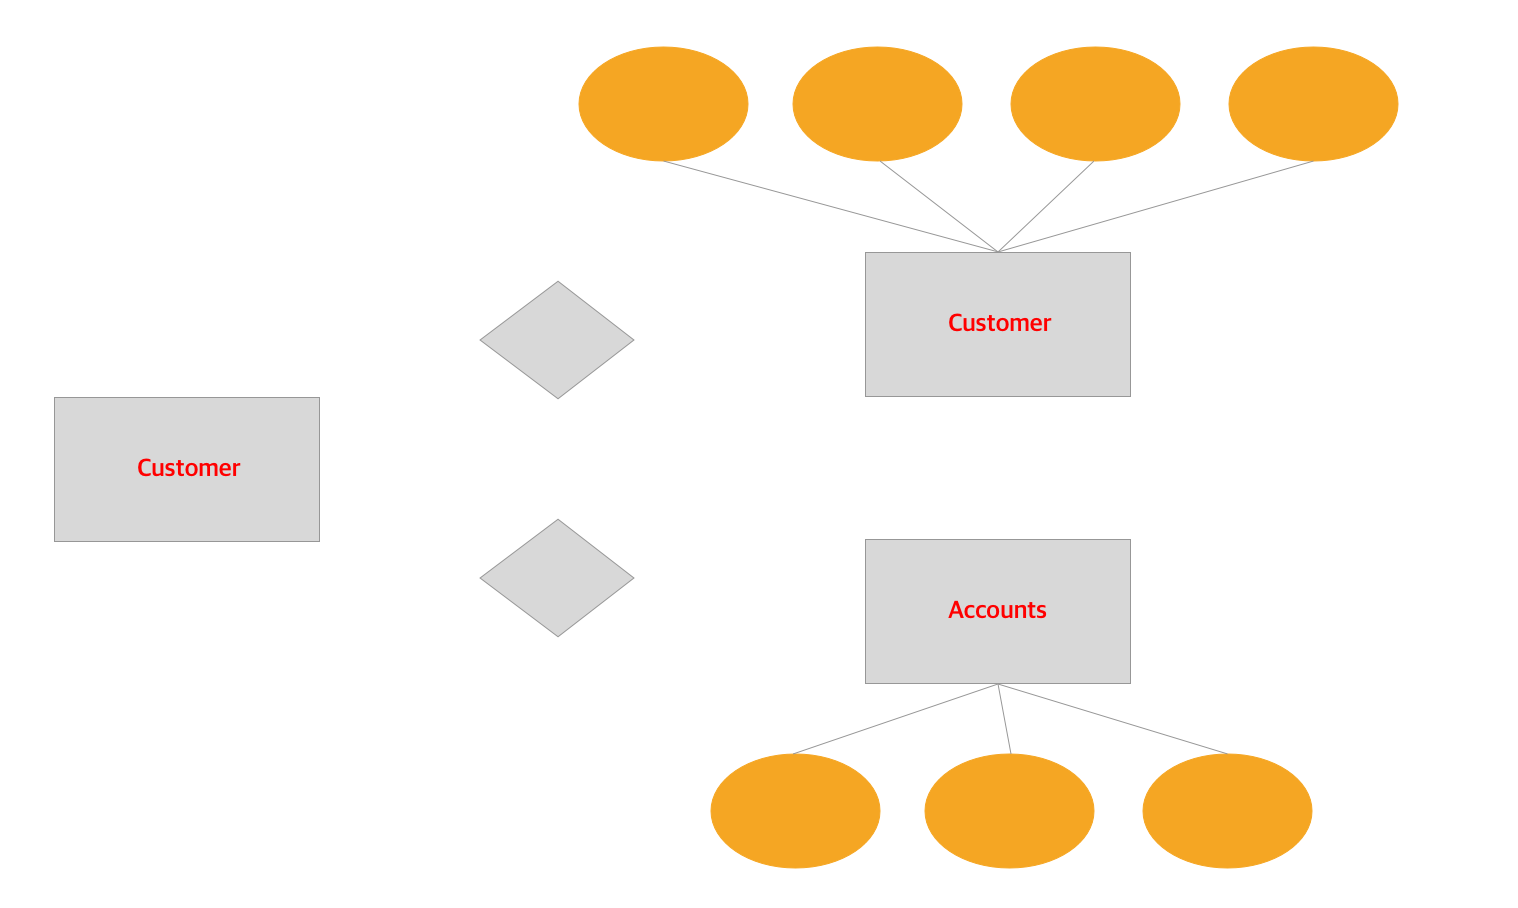
\includegraphics[width=\linewidth]{images/worksheet_14_solution_13.png}
    \end{center}

    \bigskip

    \begin{mdframed}
        \underline{\textbf{Correct Solution:}}

        \bigskip

        \begin{center}
        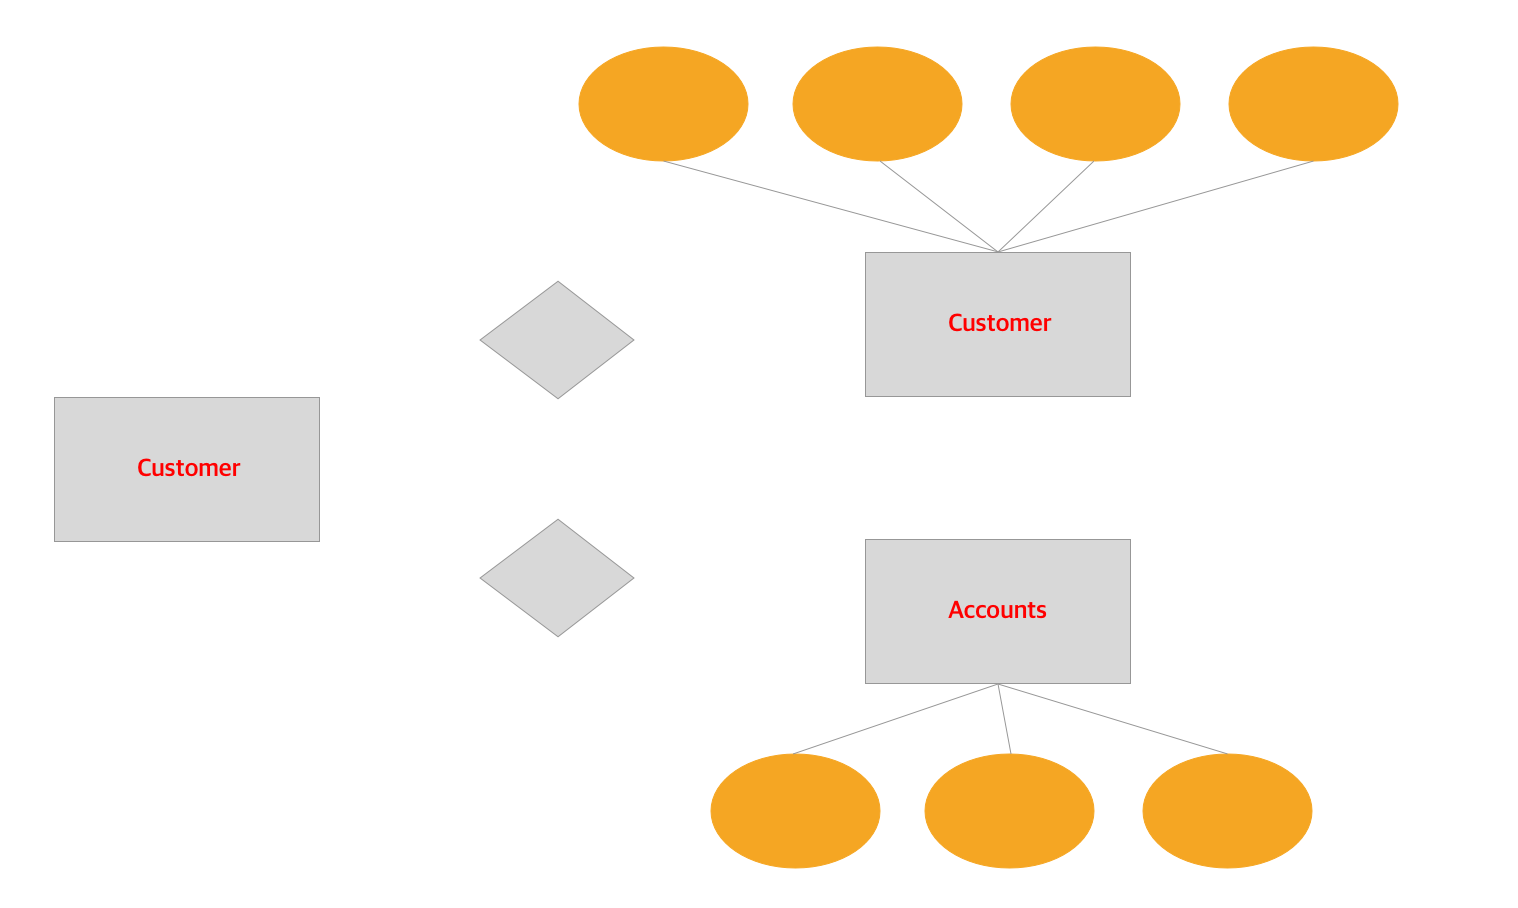
\includegraphics[width=\linewidth]{images/worksheet_14_solution_13.png}
        \end{center}

    \end{mdframed}

    \bigskip

    \underline{\textbf{Notes:}}

    \bigskip

    \begin{itemize}
        \item E/R Model
        \begin{itemize}
            \item Means \textbf{Entity Relationship Model}
            \item Entity Relationship Model(ER Modeling) is a graphical approach to database design.
            \item Is comparable to class diagram in UML
            \item Uses three principle element types:

            \begin{enumerate}[1.]
                \item Entity sets
                \begin{itemize}
                    \item Is an abstract object of some sort (i.e. entitiy)
                    \item Is not used to represent class
                    \item Is represented by rectangles
                \end{itemize}

                \begin{center}
                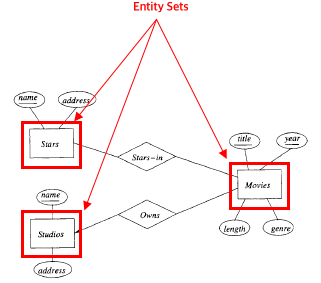
\includegraphics[width=0.7\linewidth]{images/worksheet_14_solution_1.png}
                \end{center}

                \item Attributes
                \begin{itemize}
                    \item Are properties of entities in a set (i.e. column name)
                    \item Each has its own primitive data types (e.g. String, integers, Reals)
                    \item Is represented by ovals
                \end{itemize}

                \begin{center}
                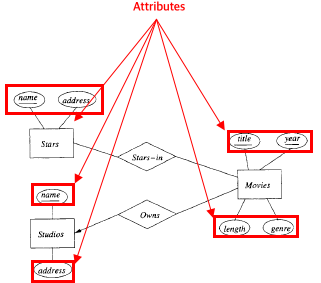
\includegraphics[width=0.7\linewidth]{images/worksheet_14_solution_2.png}
                \end{center}

                \item Relationships
                \begin{itemize}
                    \item Are connections among two or more entity sets (e.g. intermediary Relations like Stars In)
                    \item Is represented by diamond
                \end{itemize}

                \begin{center}
                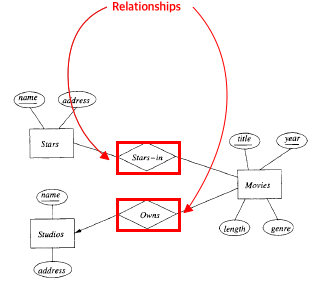
\includegraphics[width=0.7\linewidth]{images/worksheet_14_solution_3.png}
                \end{center}
            \end{enumerate}

            \bigskip

            \underline{\textbf{Example:}}

            \bigskip

            \begin{center}
            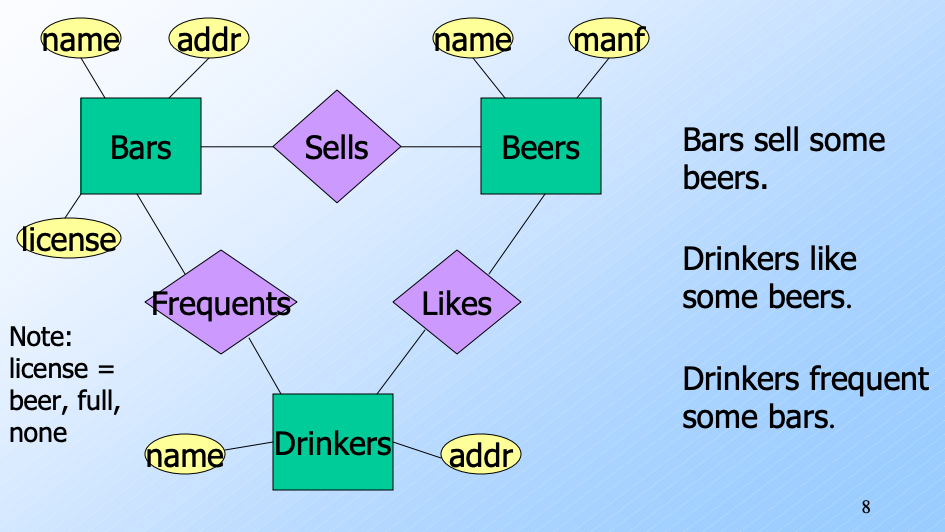
\includegraphics[width=0.7\linewidth]{images/worksheet_14_solution_4.png}
            \end{center}
        \end{itemize}

        \item Multiway Relationships

        \begin{itemize}
            \item Connects more than two relationship sets
            \item Enables to represent relationships that otherwise is
            difficult in binary relationship
            \item Arrow $\to$ 'one'
            \item No arrow $\to$ 'many'
        \end{itemize}

        \bigskip

        \underline{\textbf{Example:}}

        \bigskip

        \begin{center}
        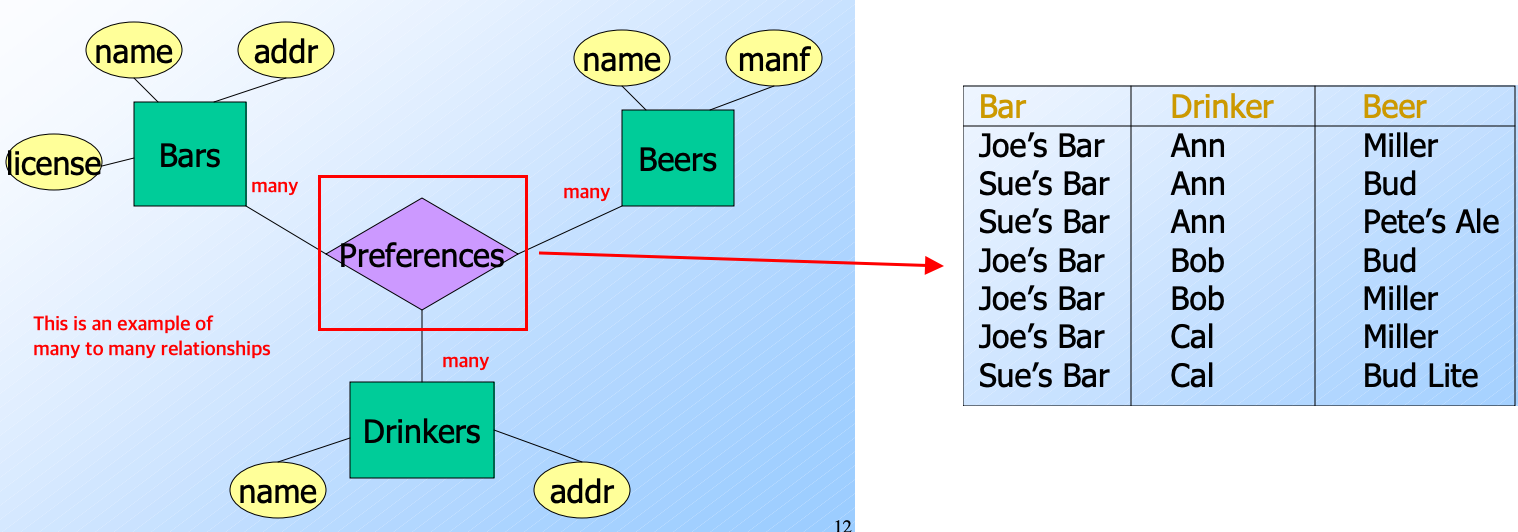
\includegraphics[width=\linewidth]{images/worksheet_14_solution_5.png}
        \end{center}

        \bigskip

        \underline{\textbf{Example 2:}}

        \bigskip

        \begin{center}
        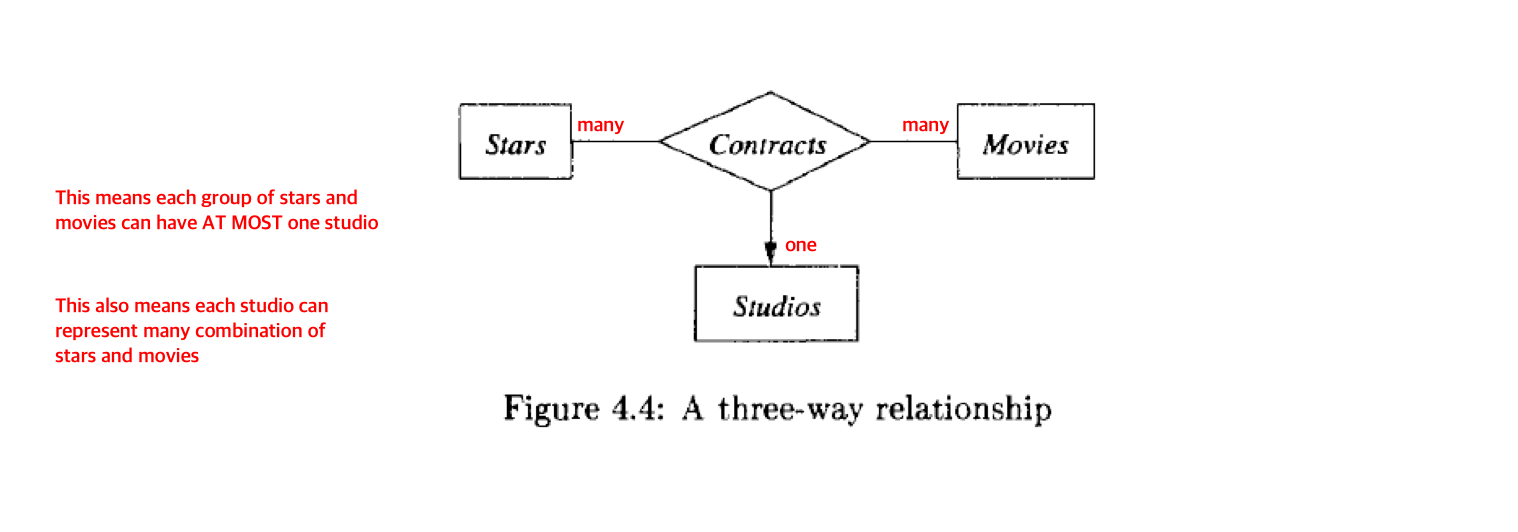
\includegraphics[width=\linewidth]{images/worksheet_14_solution_6.png}
        \end{center}

        \bigskip

        \item Roles in Relationships
        \begin{itemize}
            \item Is the label of edges between the entity set and relationship
            \item Are used to clarify the sementics of relationship
        \end{itemize}

        \bigskip

        \underline{\textbf{Example:}}

        \bigskip

        \begin{center}
        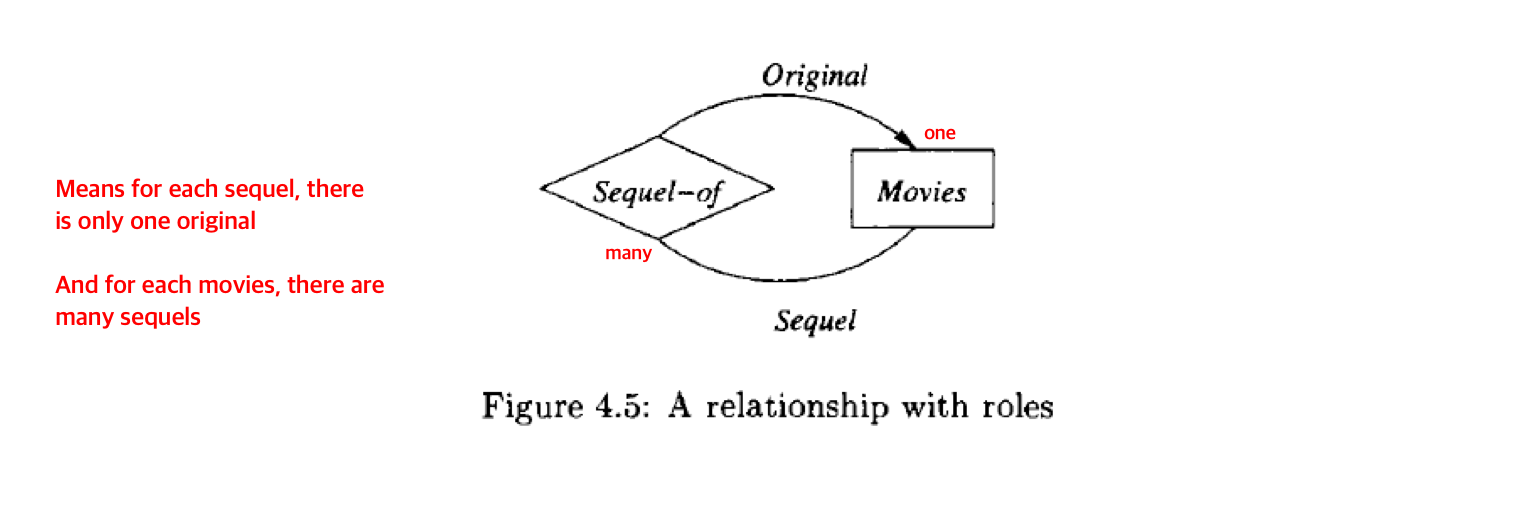
\includegraphics[width=\linewidth]{images/worksheet_14_solution_7.png}
        \end{center}

        \bigskip

        \underline{\textbf{Example 2:}}

        \bigskip

        \begin{center}
        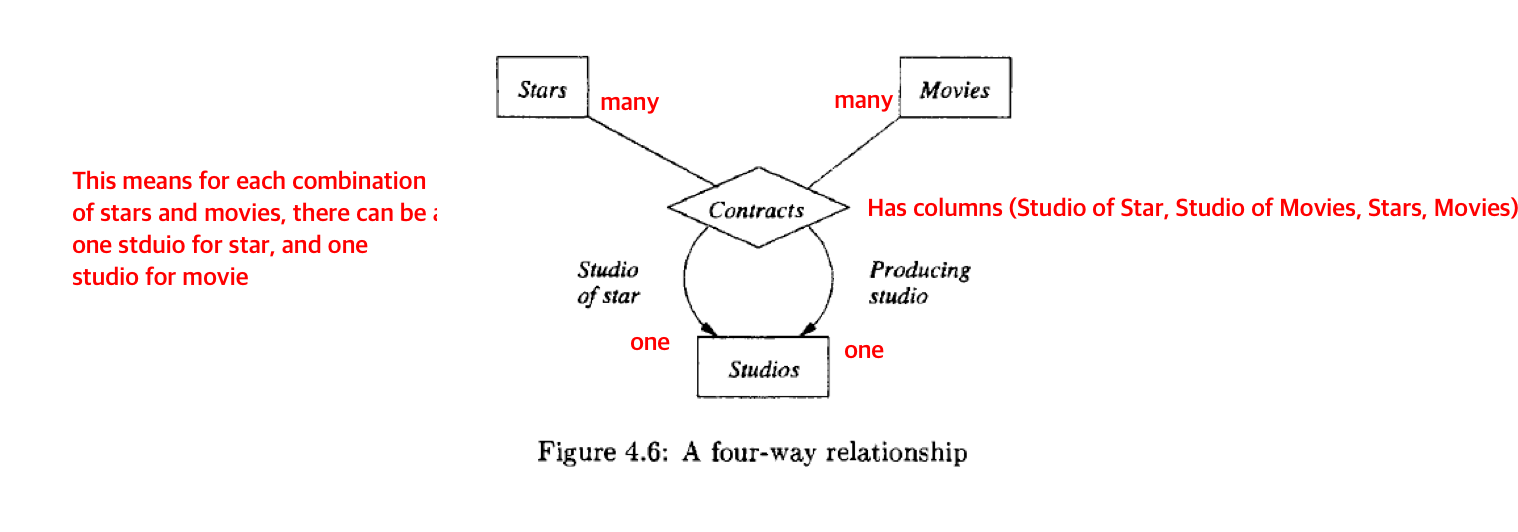
\includegraphics[width=\linewidth]{images/worksheet_14_solution_8.png}
        \end{center}

        \item Attributes on Relationships

        \begin{itemize}
            \item can be thought as a property of tuples in the relationship set
            (i.e. String, Integer, Float, Boolean)

            \bigskip

            \underline{\textbf{Example:}}

            \bigskip

            \begin{center}
            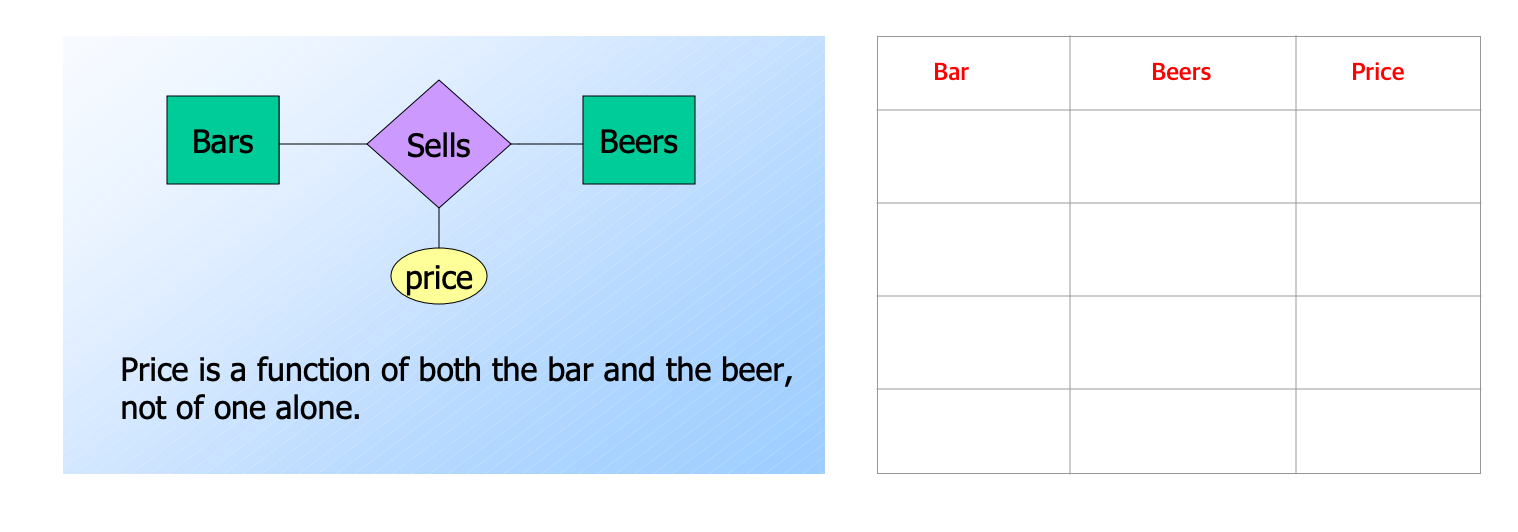
\includegraphics[width=\linewidth]{images/worksheet_14_solution_9.png}
            \end{center}

            \item Can be removed by creating an entity set with the attribute

            \bigskip

              \underline{\textbf{Example:}}

            \bigskip

            \begin{center}
            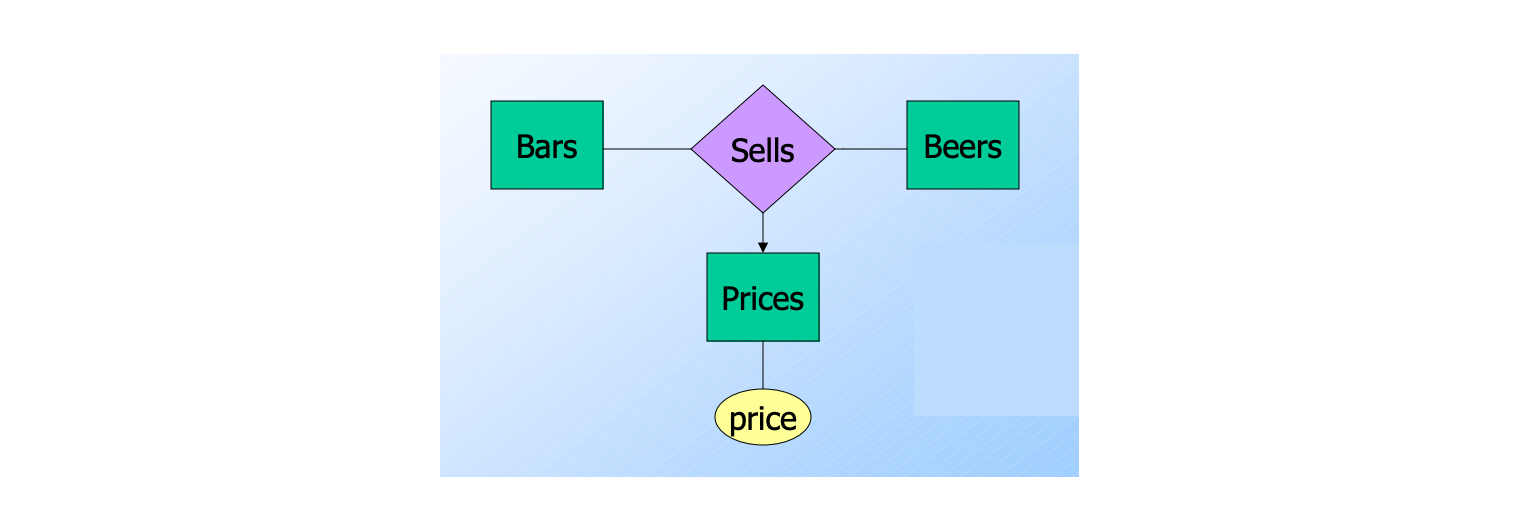
\includegraphics[width=\linewidth]{images/worksheet_14_solution_10.png}
            \end{center}
        \end{itemize}

        \item Conversting Multiway Relationships to Binary

        \bigskip

        \underline{\textbf{Example:}}

        \bigskip

        \begin{center}
        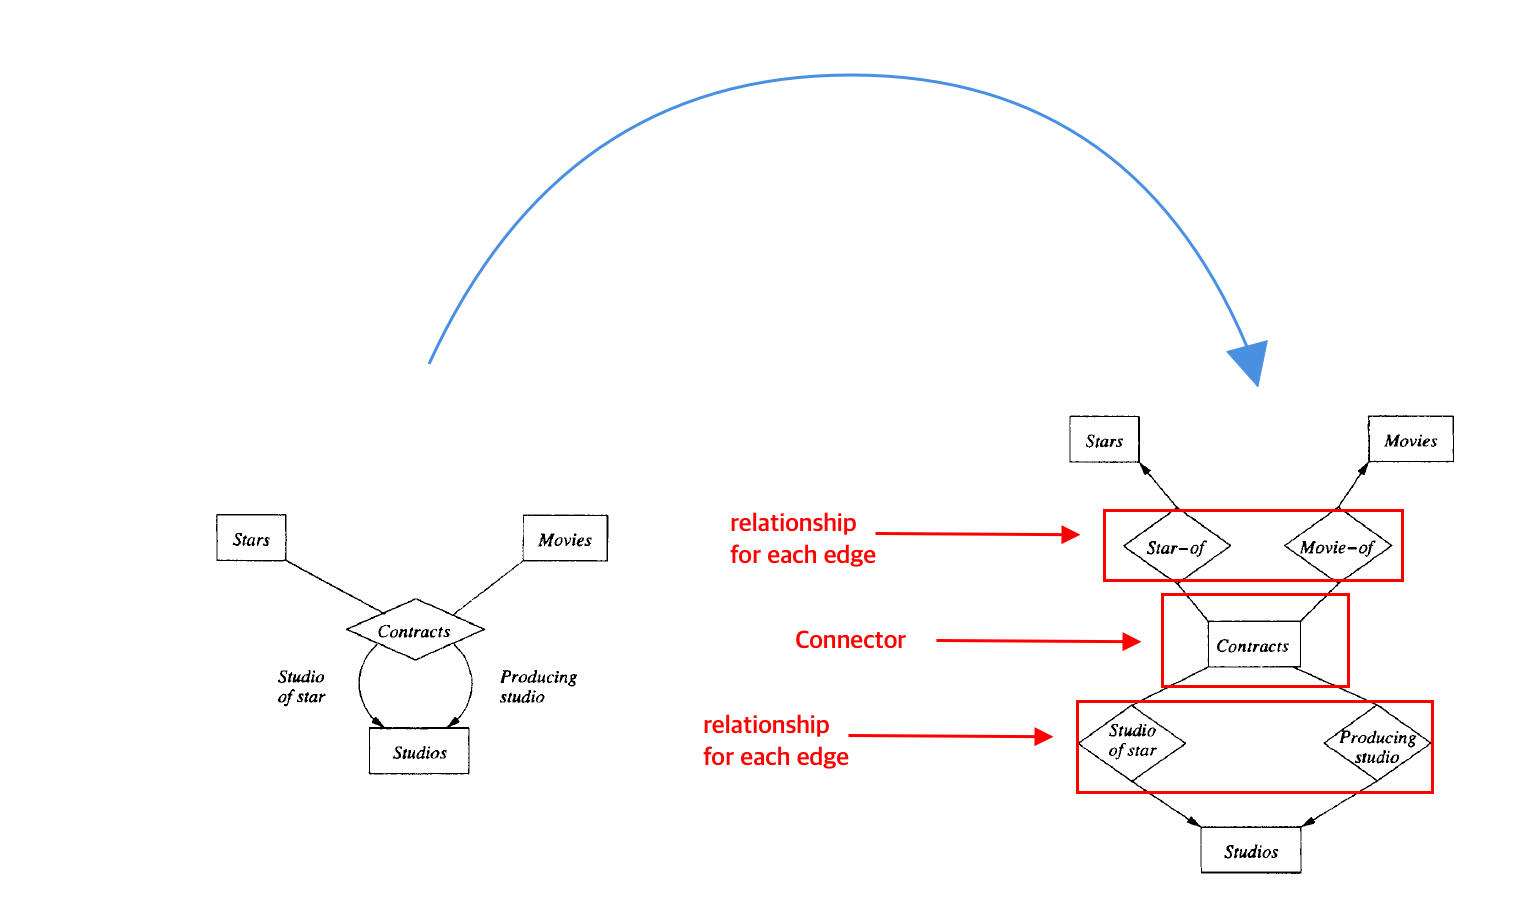
\includegraphics[width=\linewidth]{images/worksheet_14_solution_11.png}
        \end{center}


        \item Subclasses in the E/R Model

        \begin{itemize}
            \item Has its own special attributes and/or relationships
            \item All `\textit{isa}' relationship is \underline{one to one}
            \item Is represented by triangle with label `\textit{isa}' followed by
            entity set
        \end{itemize}

        \bigskip

        \underline{\textbf{Example:}}

        \bigskip

        \begin{center}
        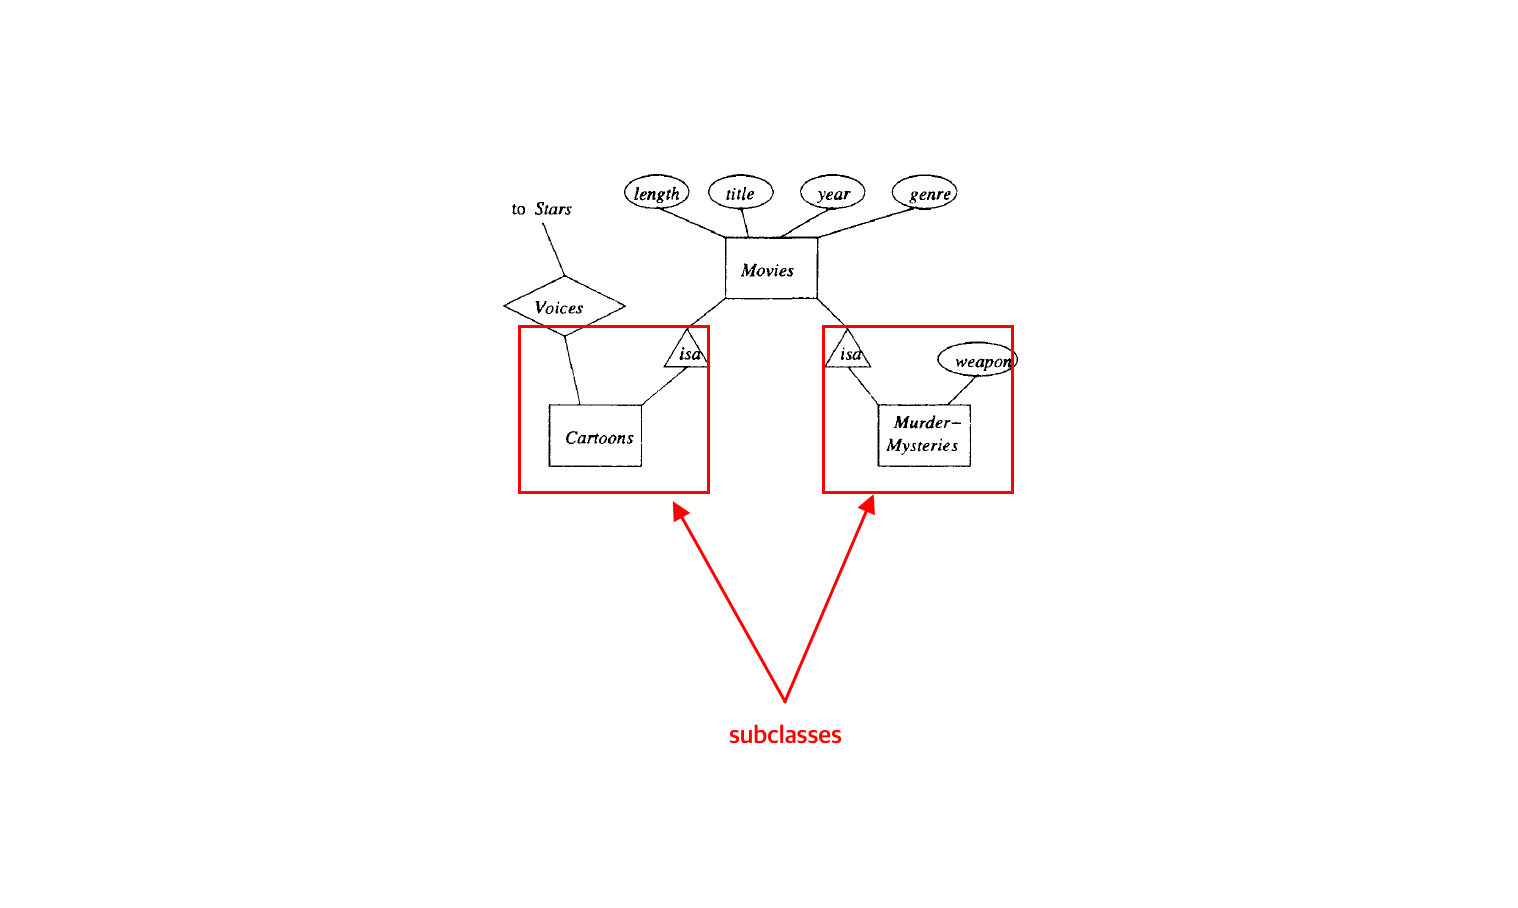
\includegraphics[width=\linewidth]{images/worksheet_14_solution_12.png}
        \end{center}

        \bigskip



    \end{itemize}

    \item

    \begin{enumerate}[a)]
        \item

        \begin{center}
        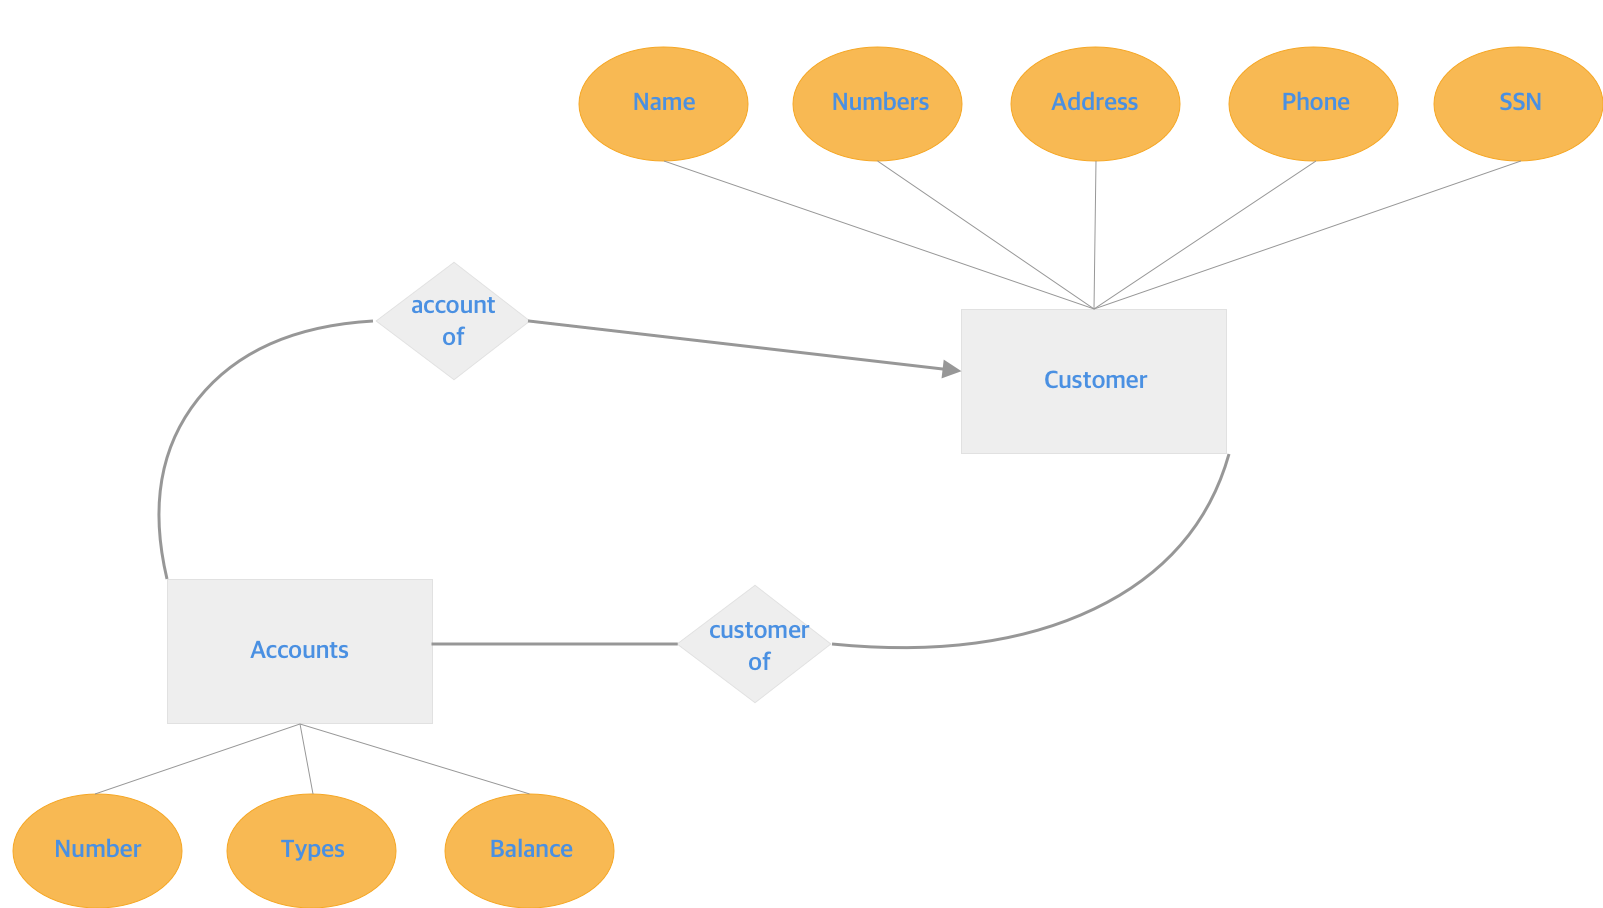
\includegraphics[width=\linewidth]{images/worksheet_14_solution_15.png}
        \end{center}

        \bigskip

        \begin{mdframed}
            \underline{\textbf{Correct Solution:}}

            \bigskip

            \begin{center}
            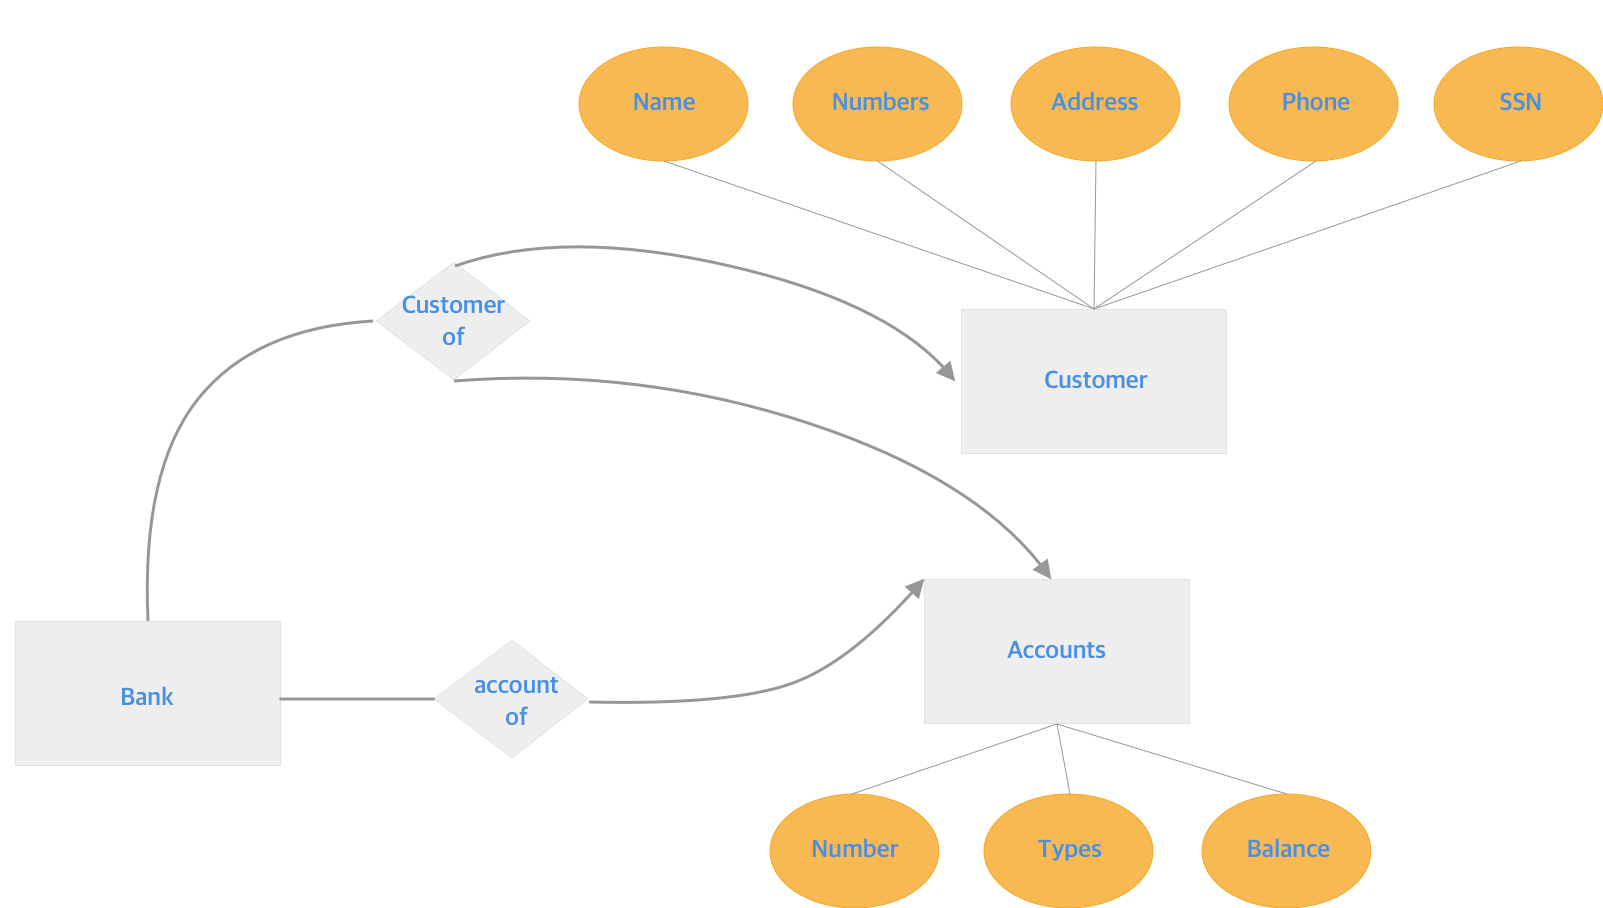
\includegraphics[width=\linewidth]{images/worksheet_14_solution_17.png}
            \end{center}
        \end{mdframed}

        \item

        \begin{center}
        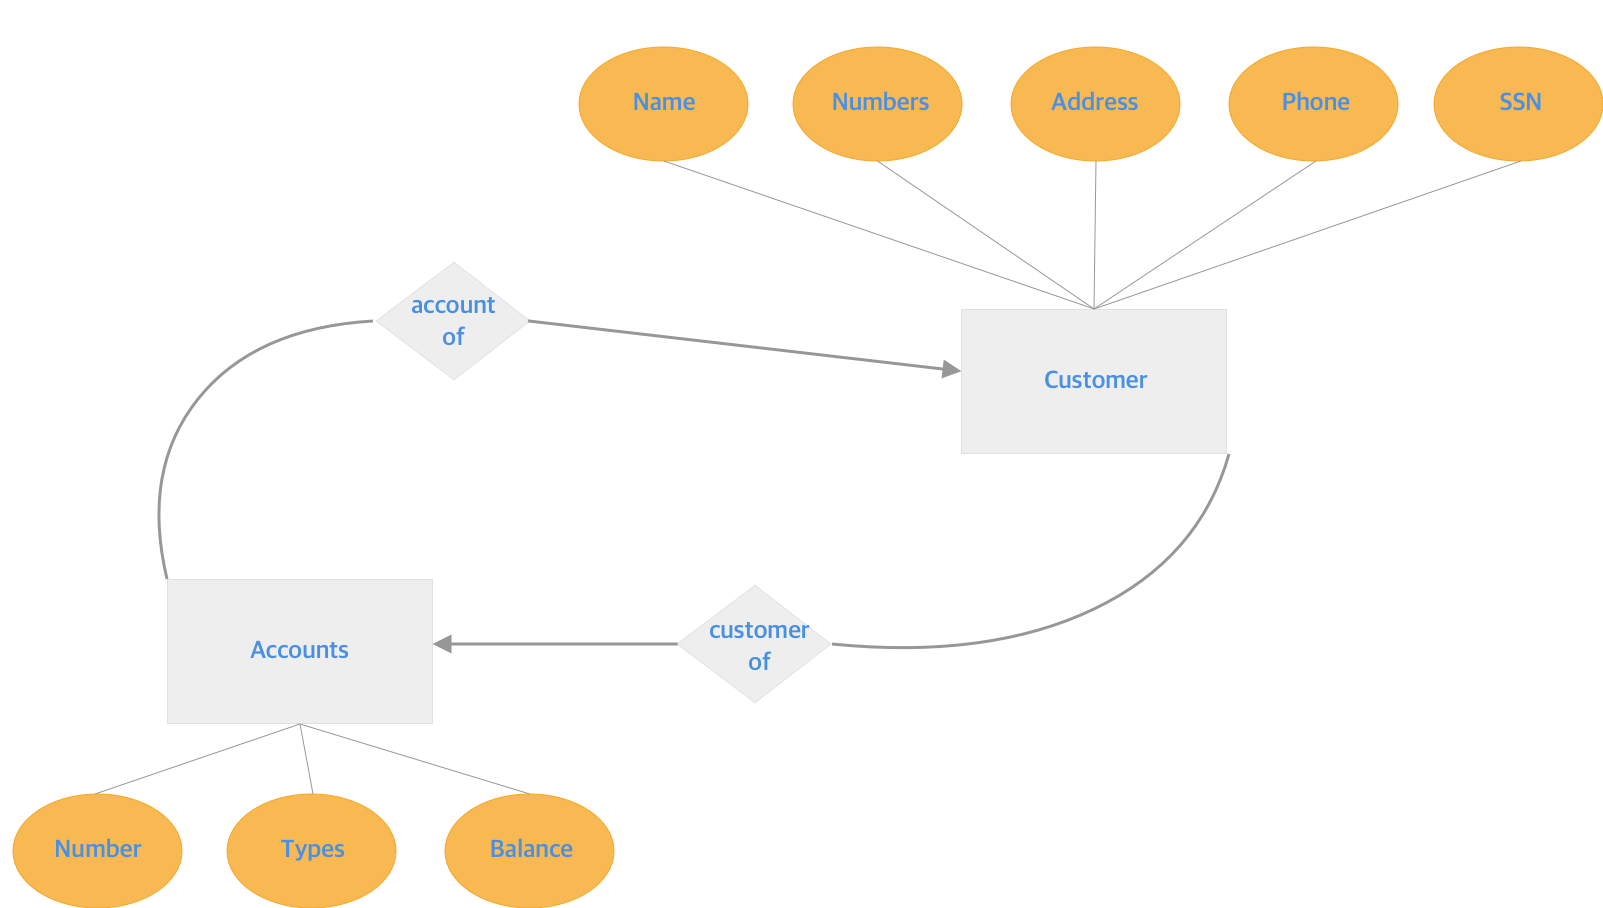
\includegraphics[width=\linewidth]{images/worksheet_14_solution_16.png}
        \end{center}

        \bigskip

        \begin{mdframed}
            \underline{\textbf{Correct Solution:}}

            \bigskip

            \begin{center}
            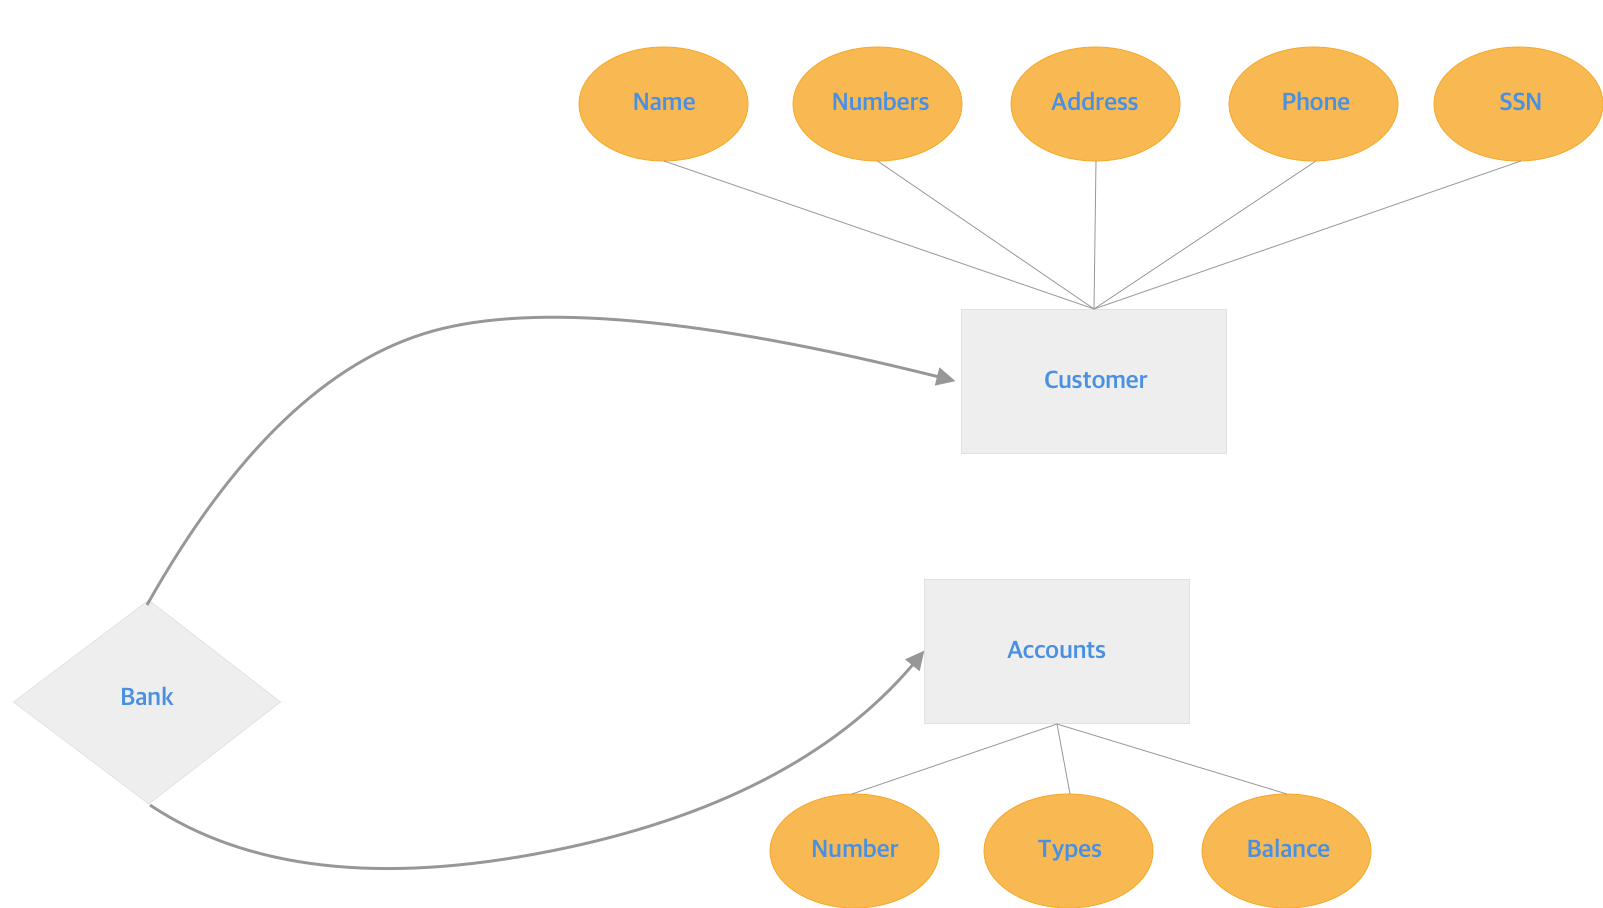
\includegraphics[width=\linewidth]{images/worksheet_14_solution_18.png}
            \end{center}
        \end{mdframed}

        \item

        \begin{center}
        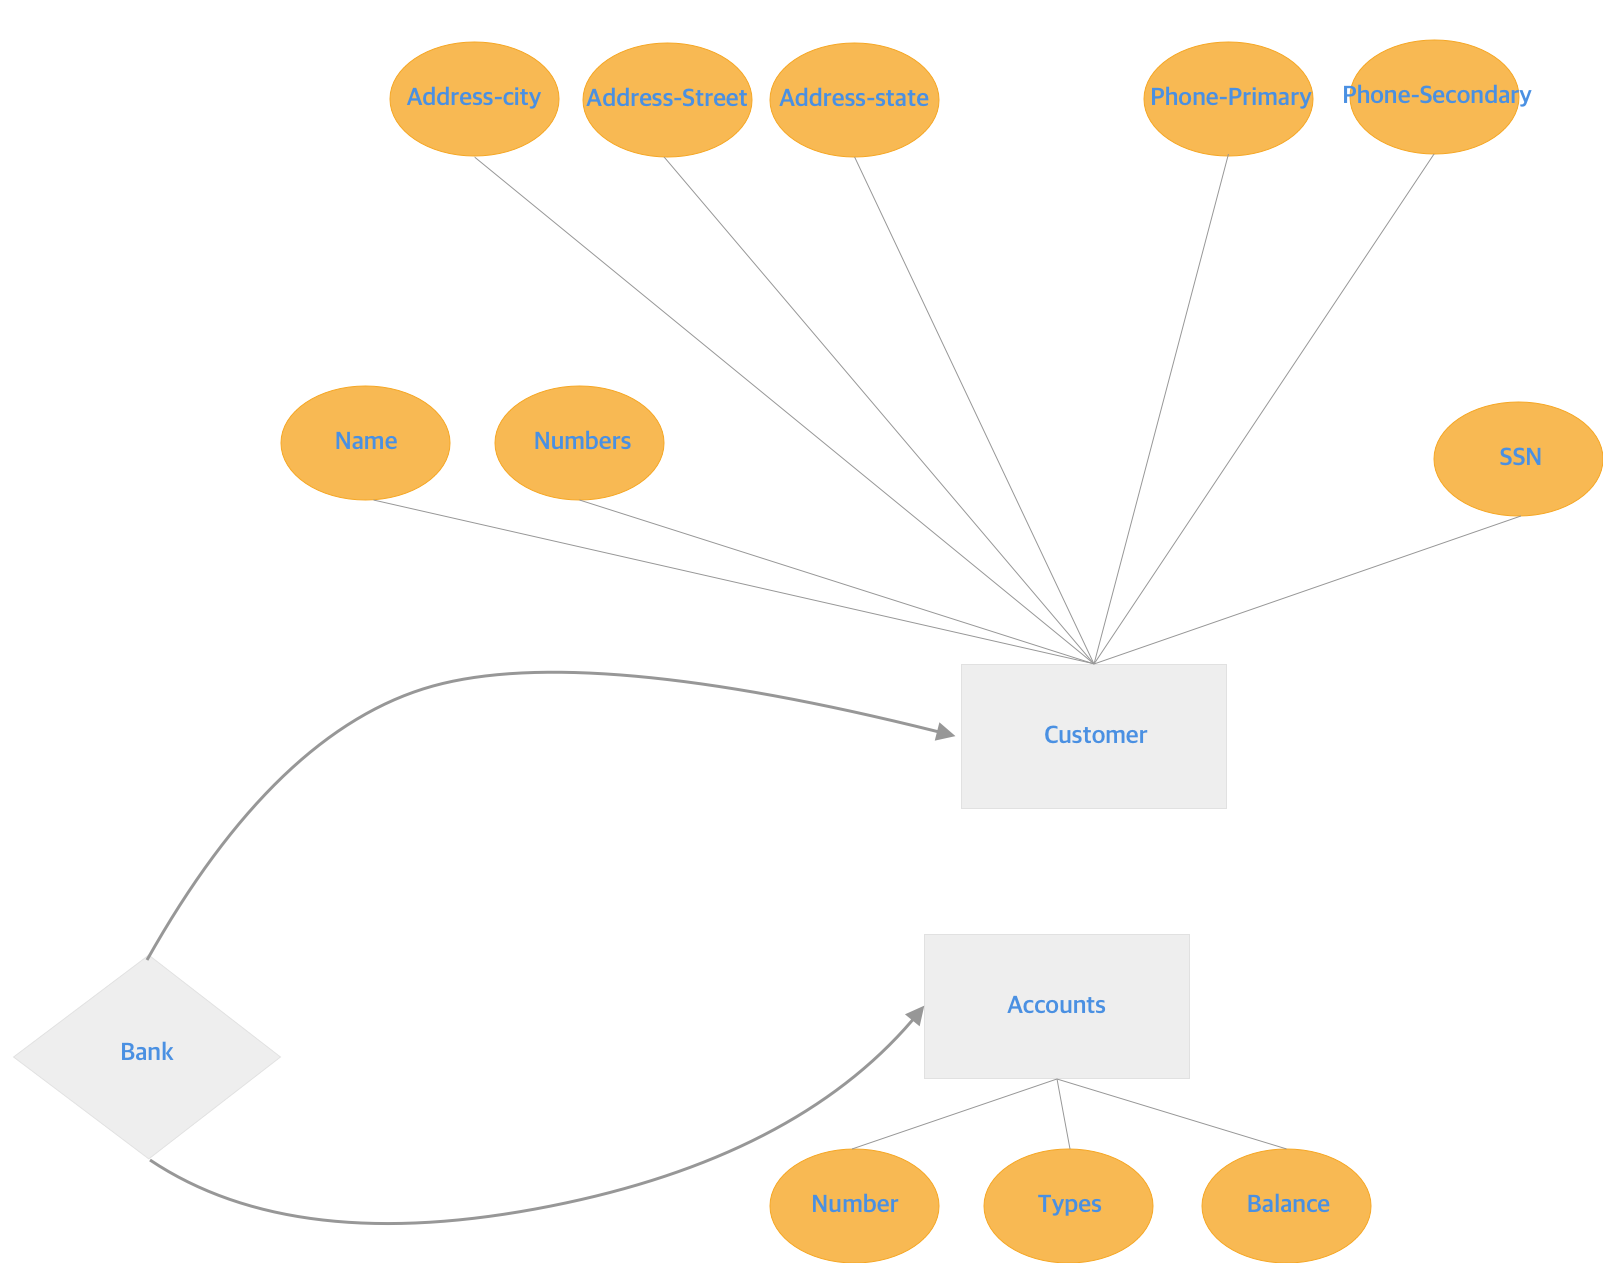
\includegraphics[width=\linewidth]{images/worksheet_14_solution_19.png}
        \end{center}

        \bigskip

        \begin{mdframed}
            \underline{\textbf{Correct Solution:}}

            \bigskip

            \begin{center}
            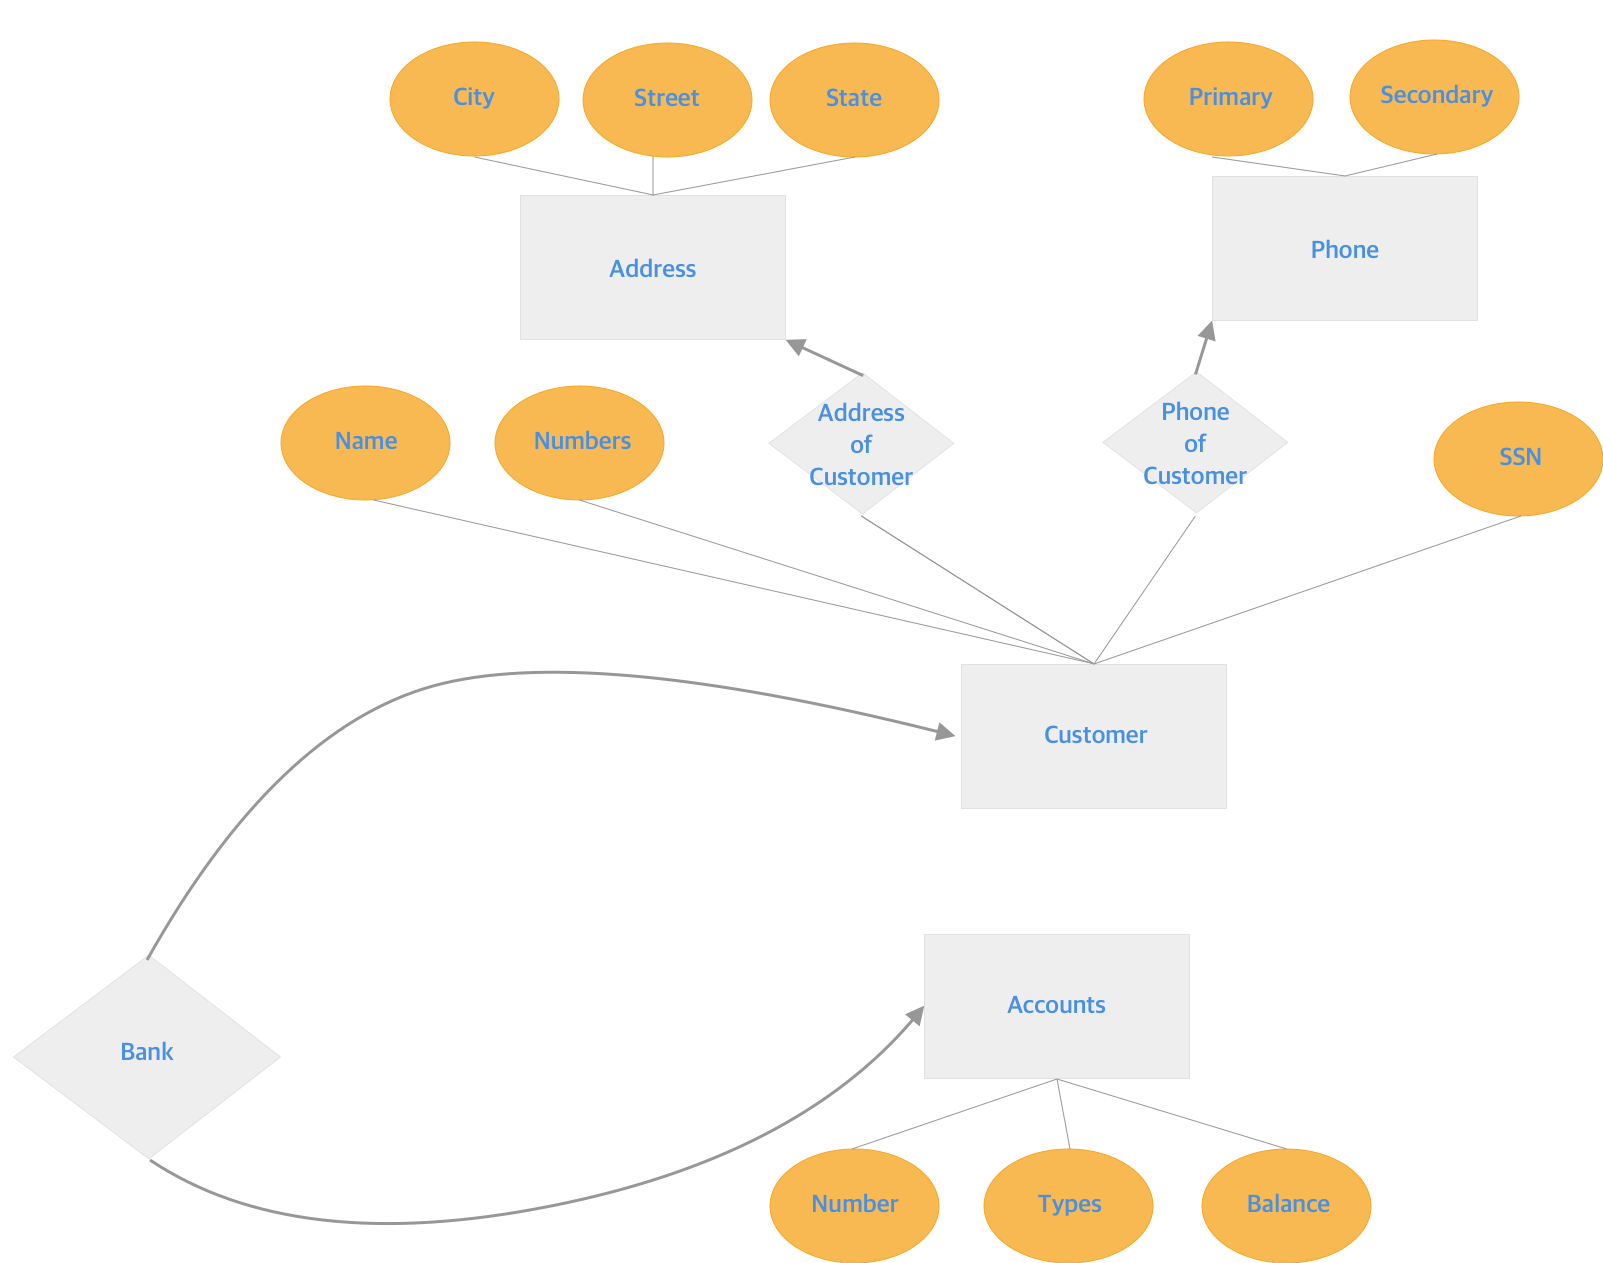
\includegraphics[width=\linewidth]{images/worksheet_14_solution_20.png}
            \end{center}

        \end{mdframed}

        \item

        \begin{center}
        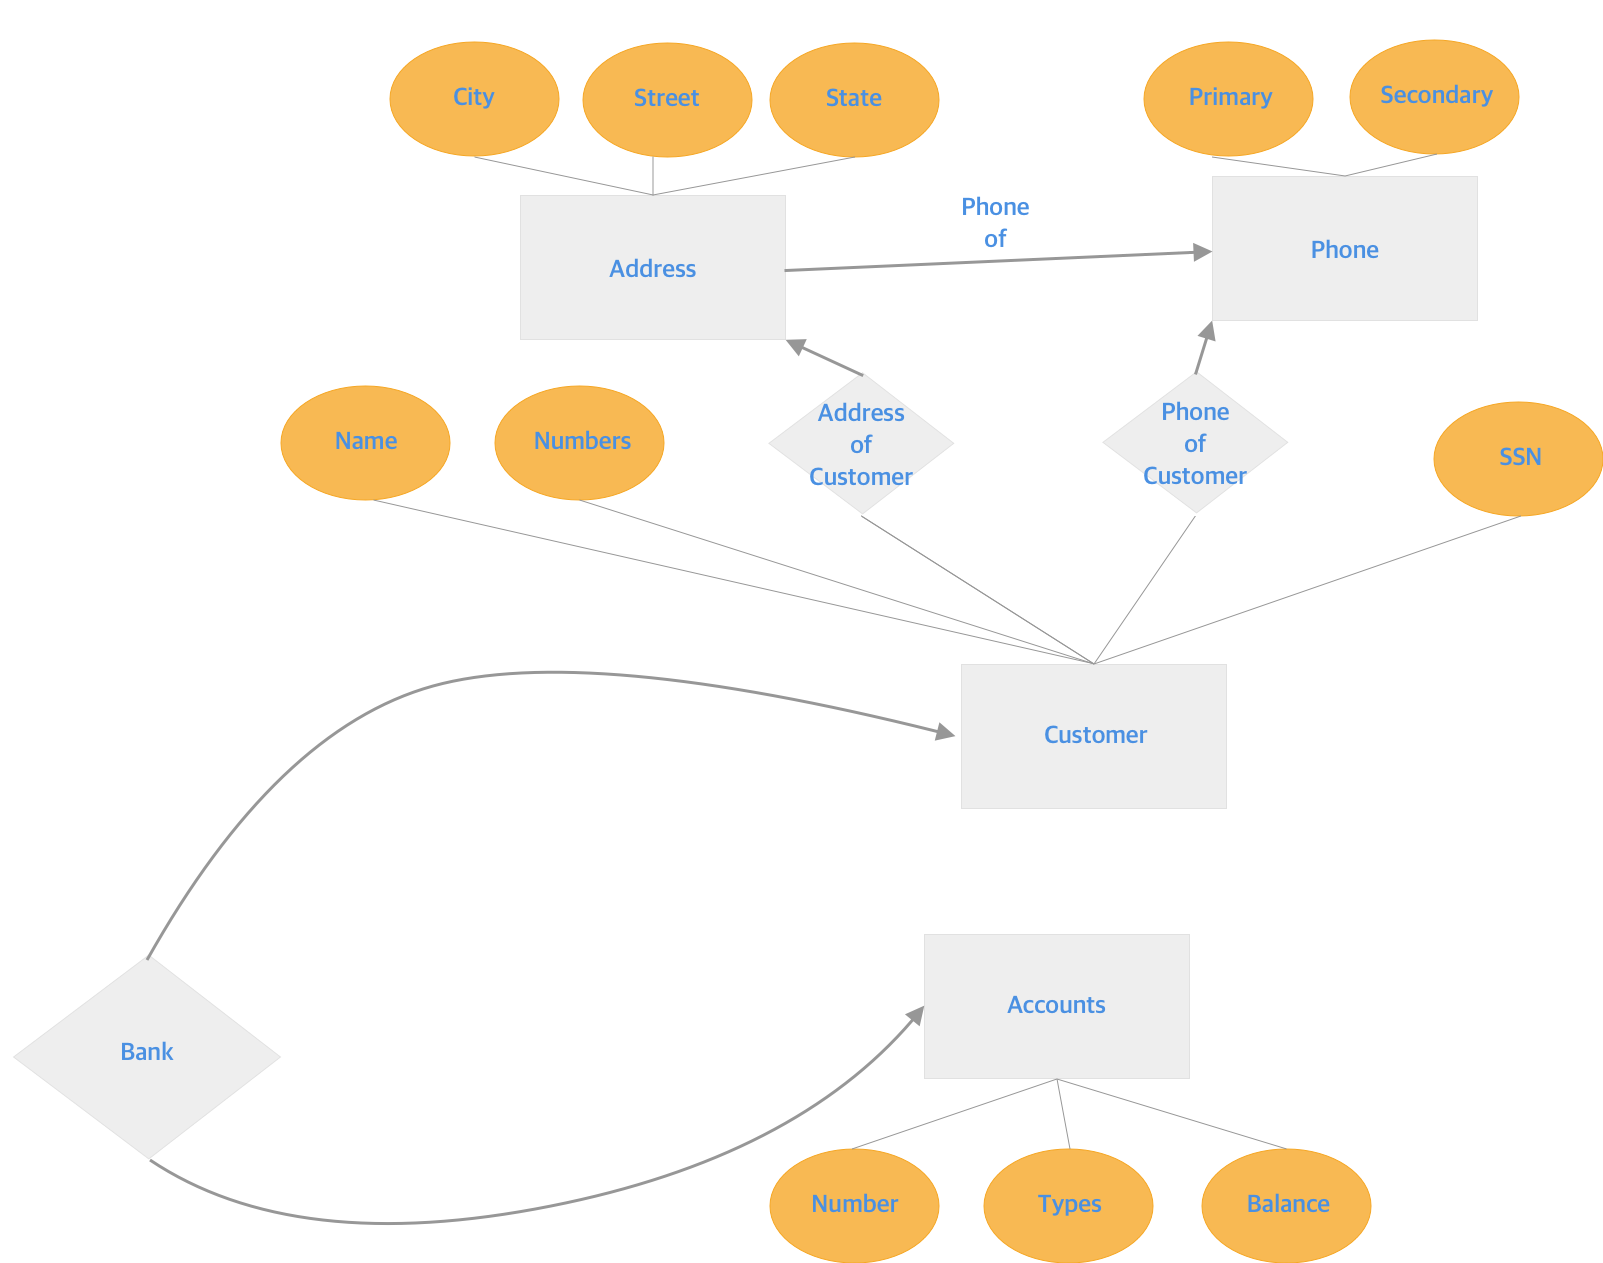
\includegraphics[width=\linewidth]{images/worksheet_14_solution_21.png}
        \end{center}

        \bigskip

        \begin{mdframed}
            \underline{\textbf{Correct Solution:}}

            \bigskip

            \begin{center}
            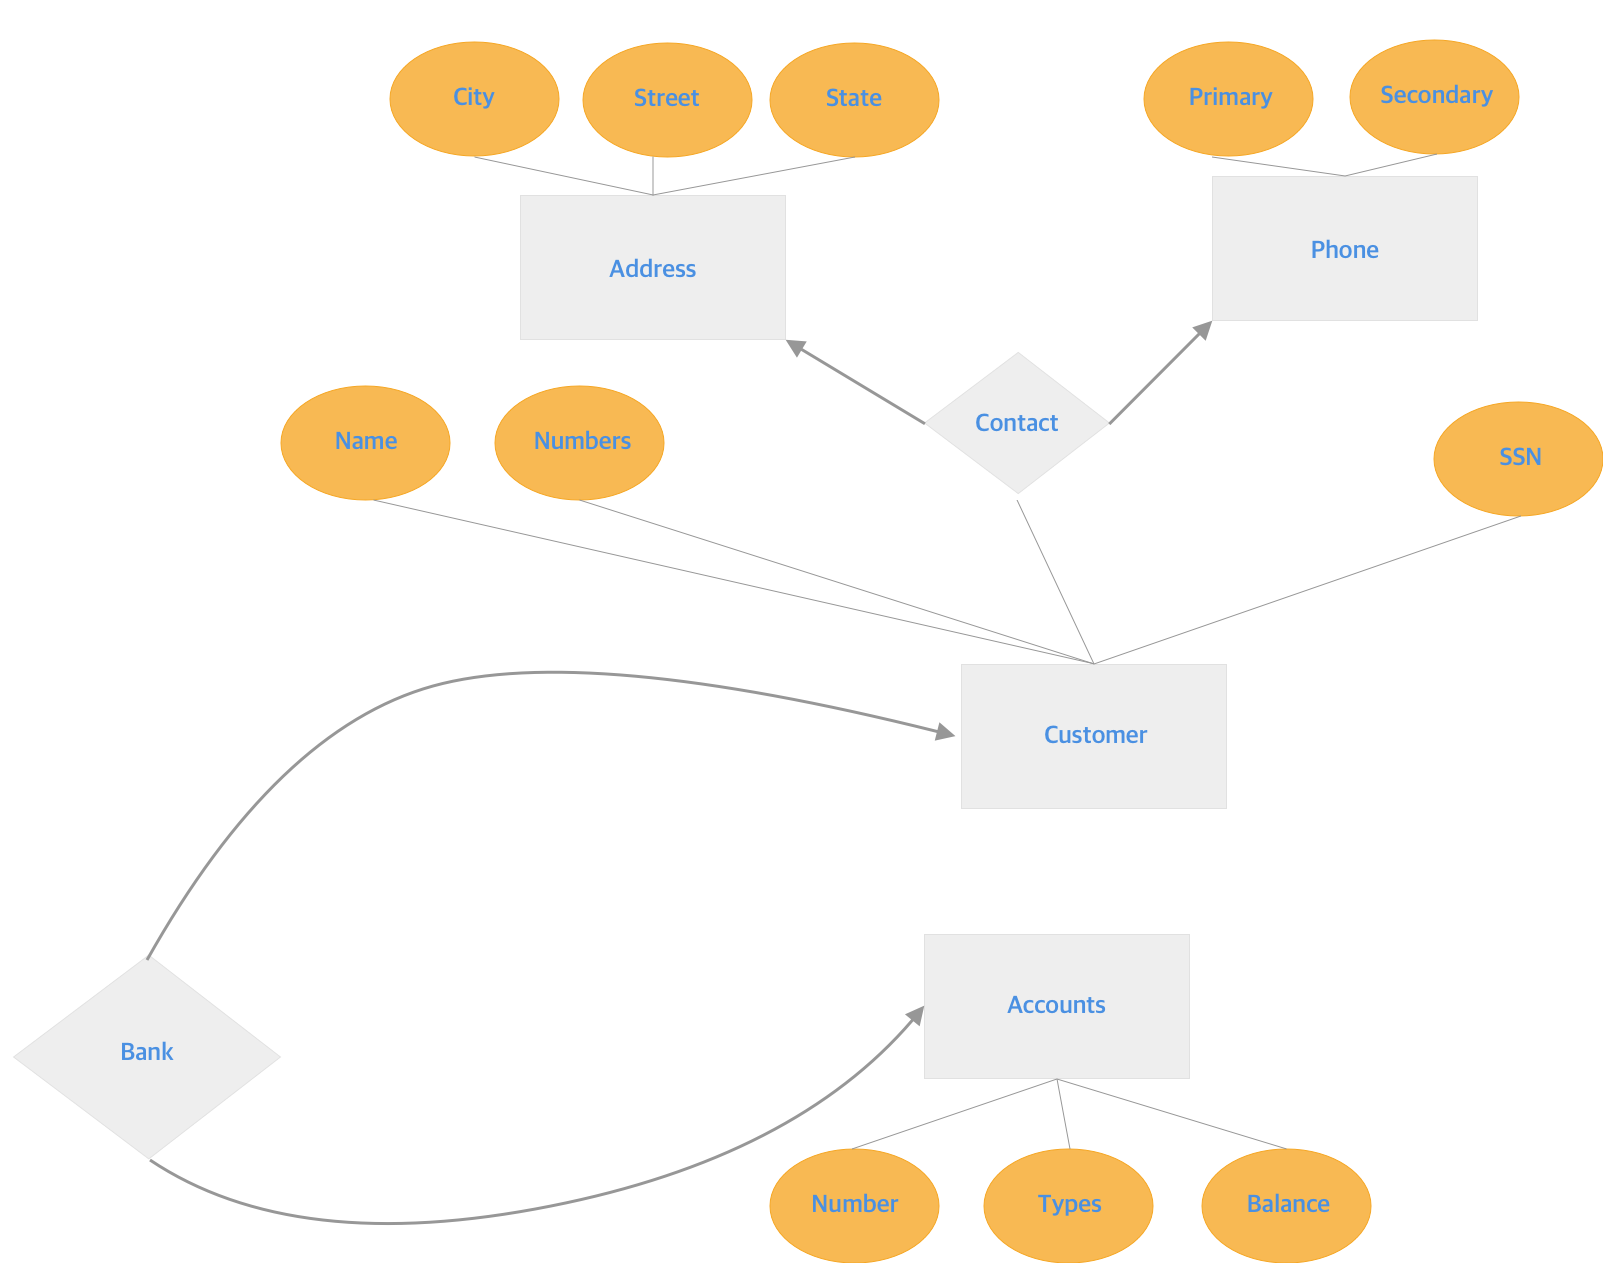
\includegraphics[width=\linewidth]{images/worksheet_14_solution_22.png}
            \end{center}

        \end{mdframed}

    \end{enumerate}

    \item

    \begin{center}
    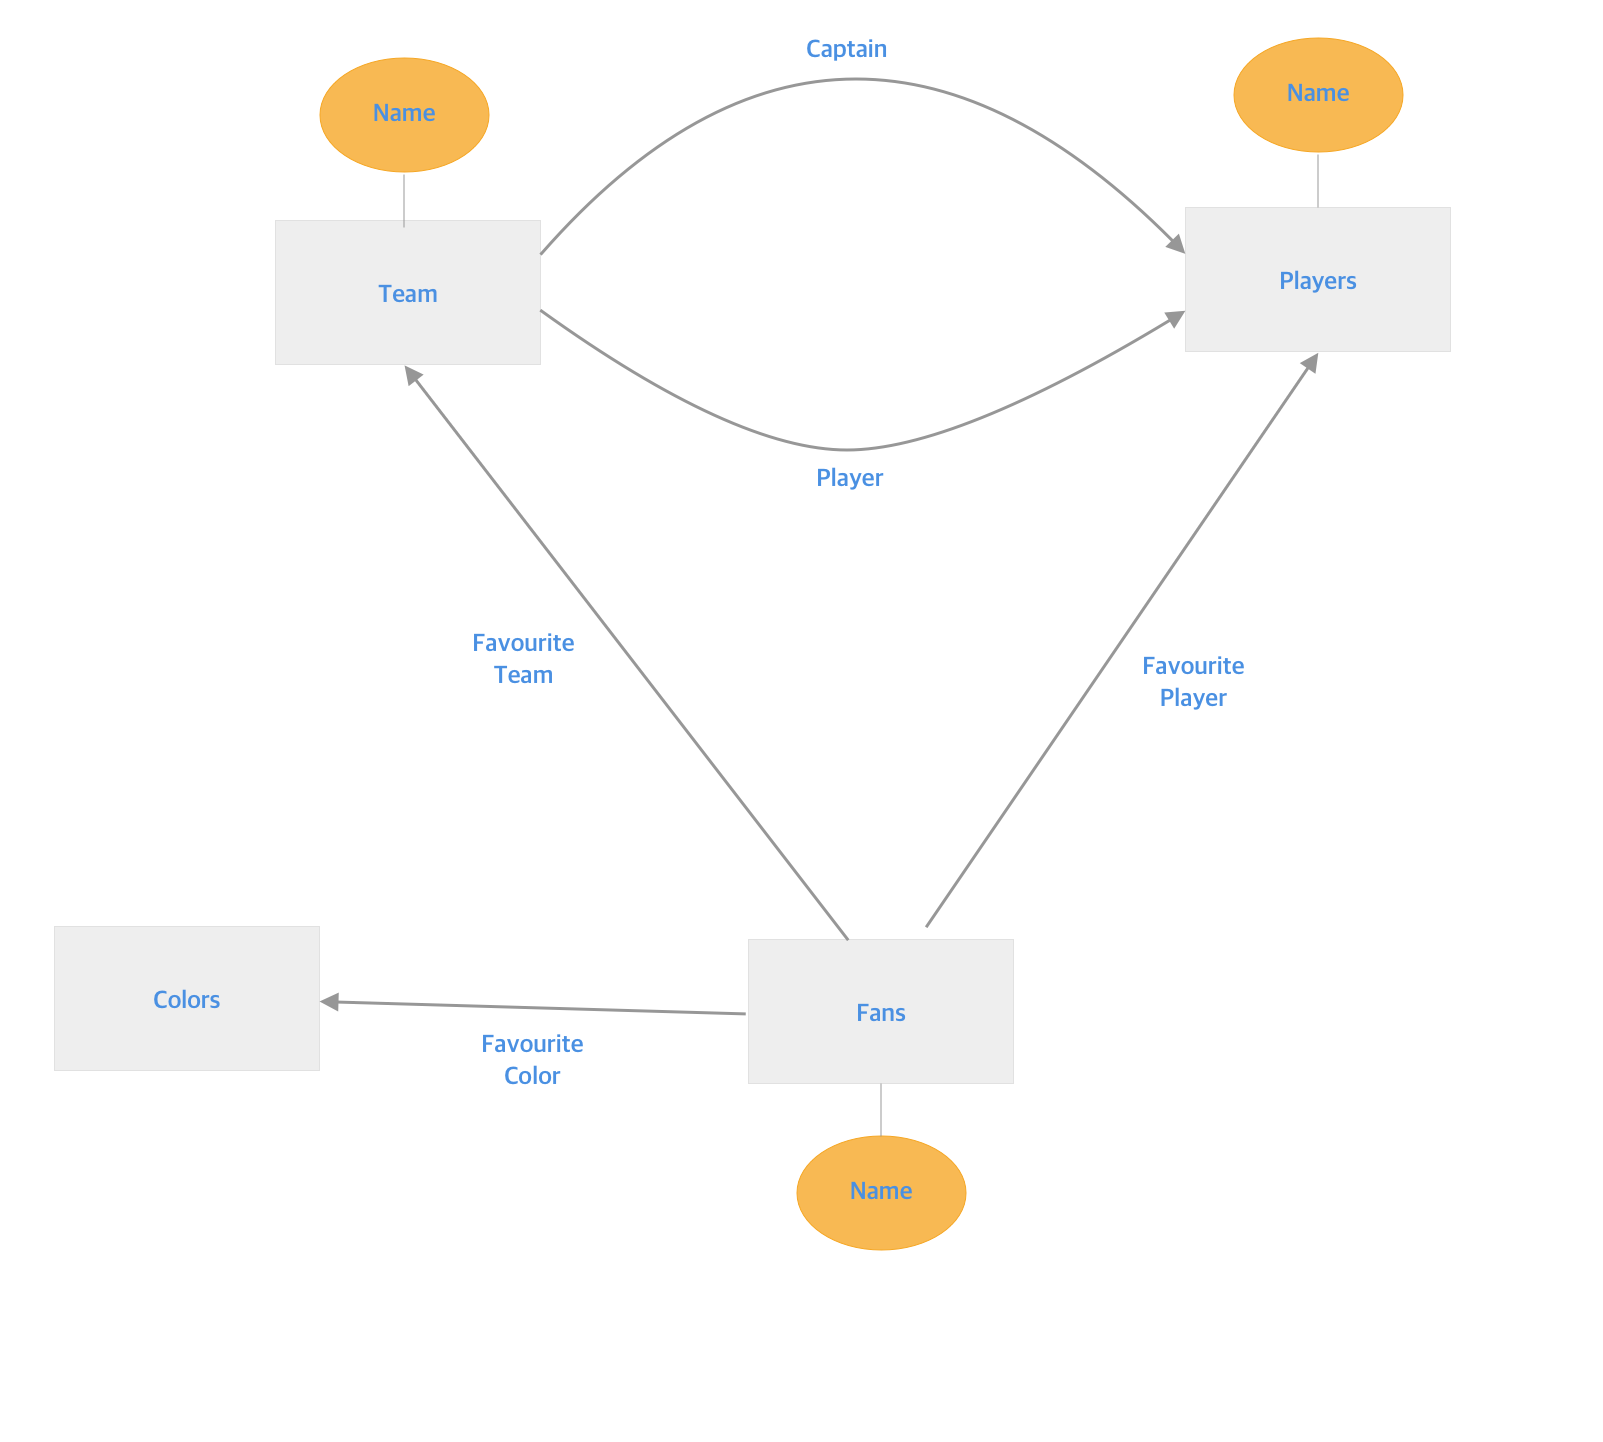
\includegraphics[width=\linewidth]{images/worksheet_14_solution_23.png}
    \end{center}

    \bigskip

    \begin{mdframed}

        \underline{\textbf{Correct Solution}}

        \bigskip

        \begin{center}
        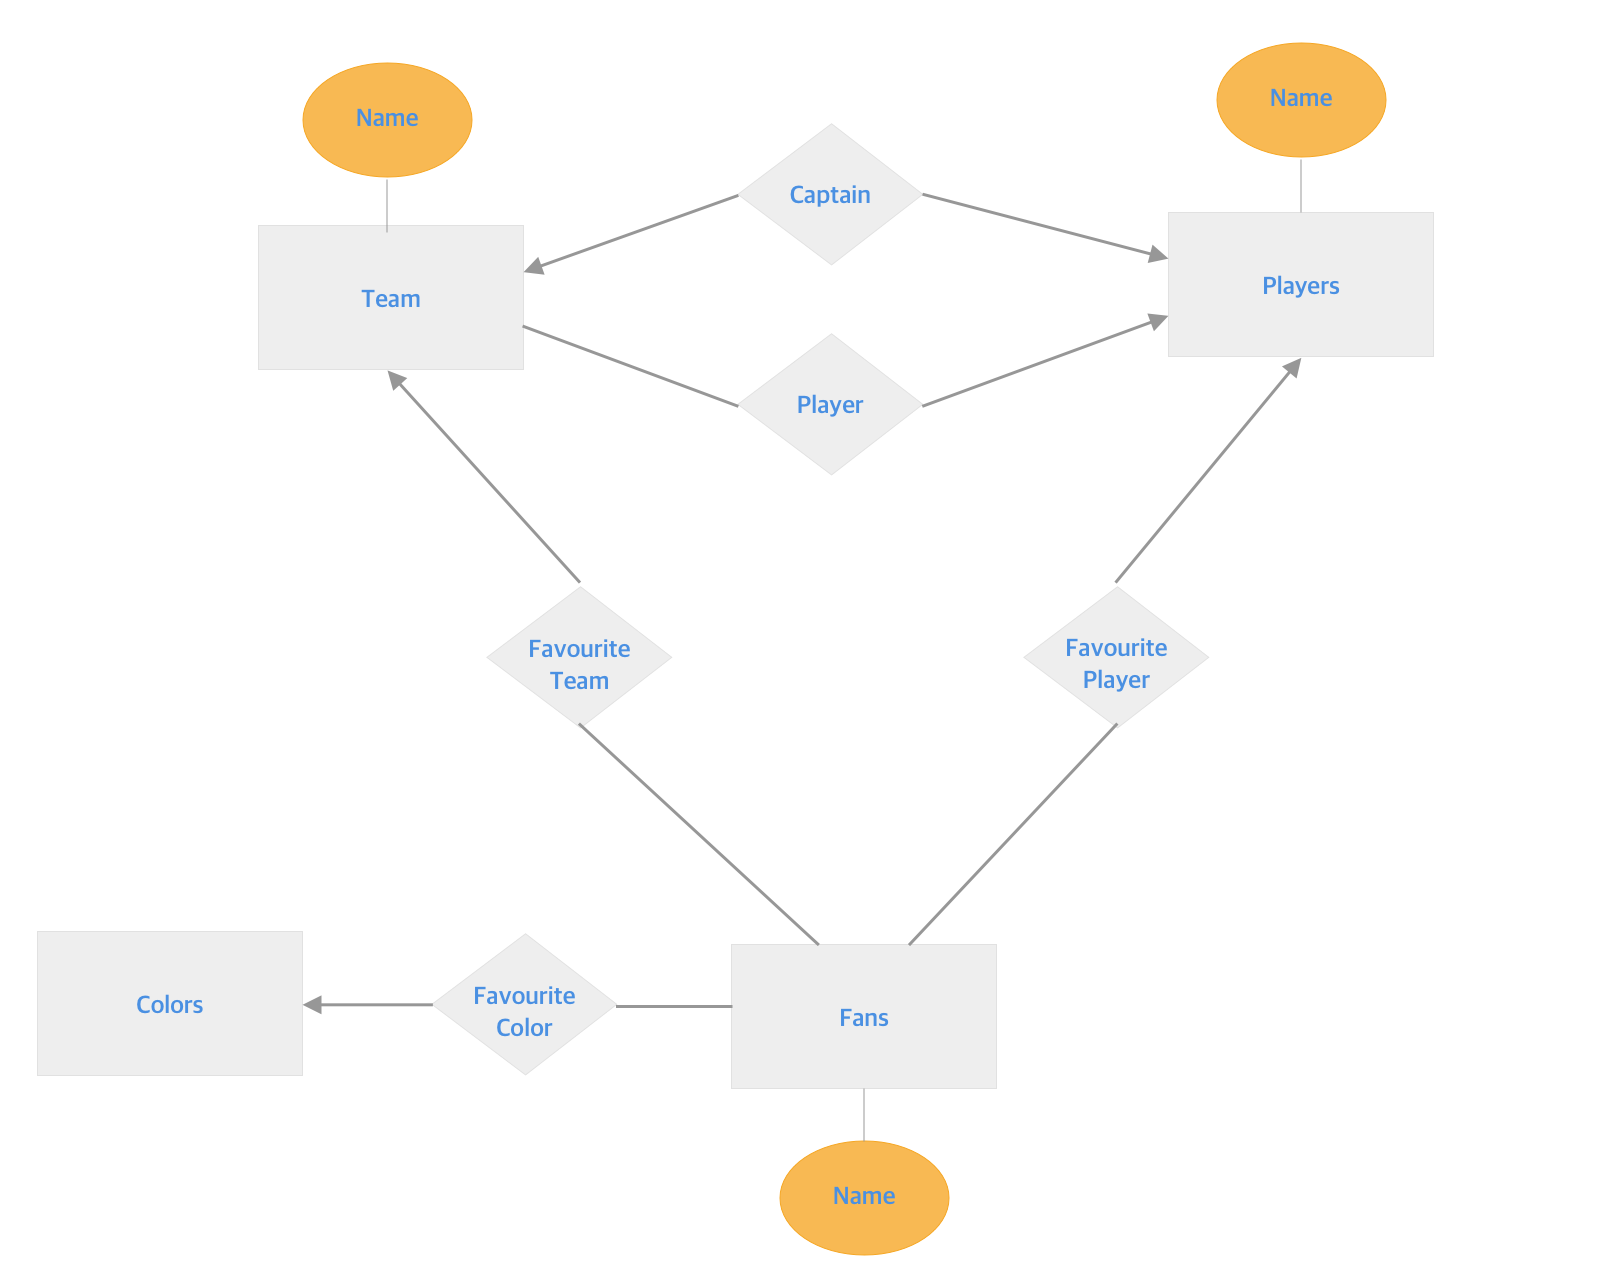
\includegraphics[width=\linewidth]{images/worksheet_14_solution_24.png}
        \end{center}

    \end{mdframed}

    \item


    \begin{enumerate}[a)]
        \item

        \begin{center}
        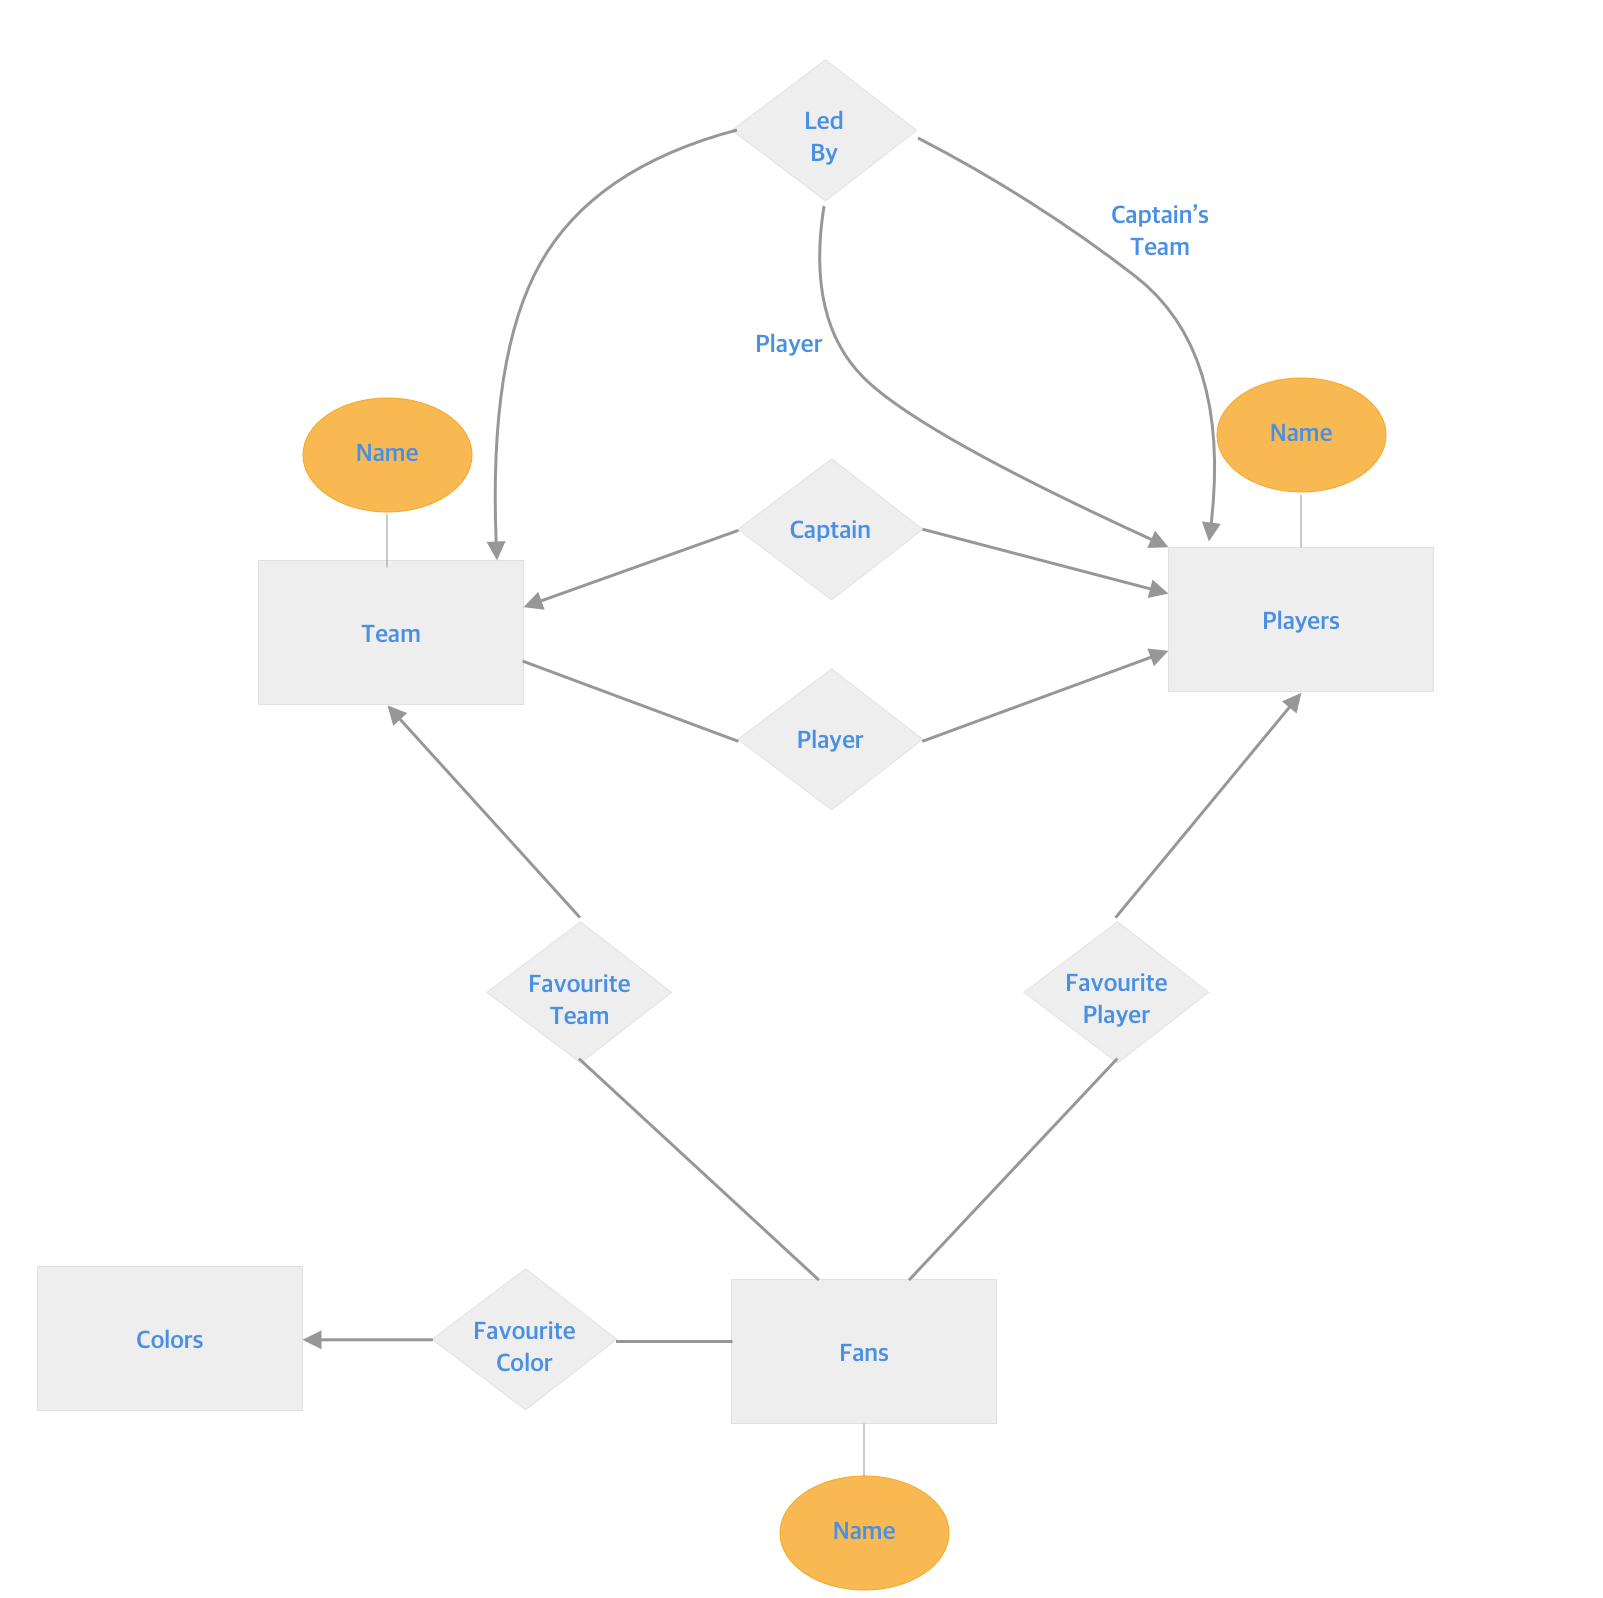
\includegraphics[width=\linewidth]{images/worksheet_14_solution_25.png}
        \end{center}

        \item

        \begin{center}
        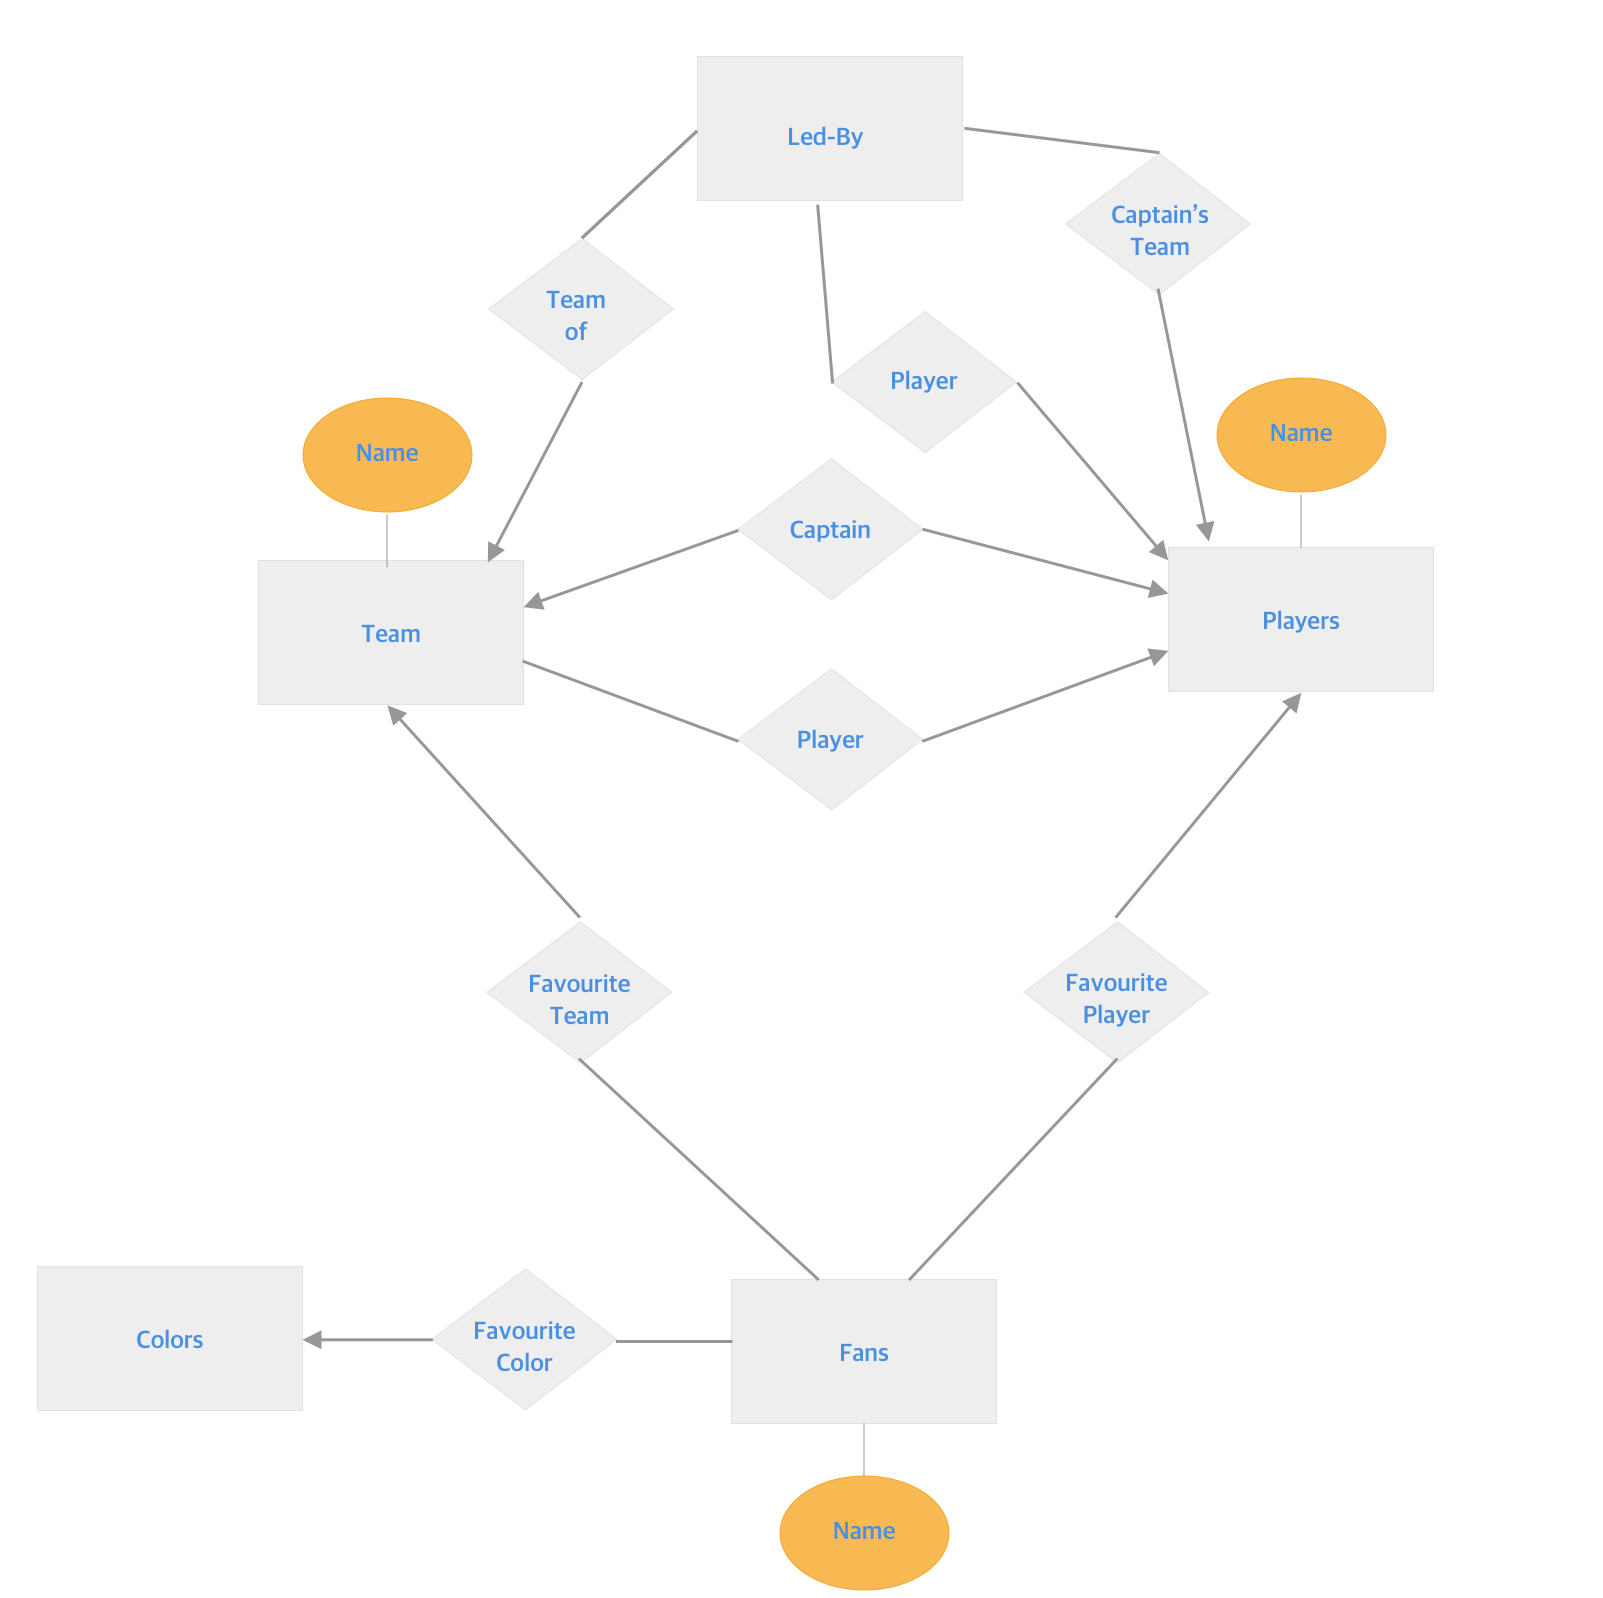
\includegraphics[width=\linewidth]{images/worksheet_14_solution_26.png}
        \end{center}

        \item

        They are the same. (I need more work on providing reason).


        \bigskip

        \underline{\textbf{Notes:}}

        \bigskip

        \begin{itemize}
            \item I should ask professor about this :'(
        \end{itemize}


    \end{enumerate}

    \item

    \begin{center}
    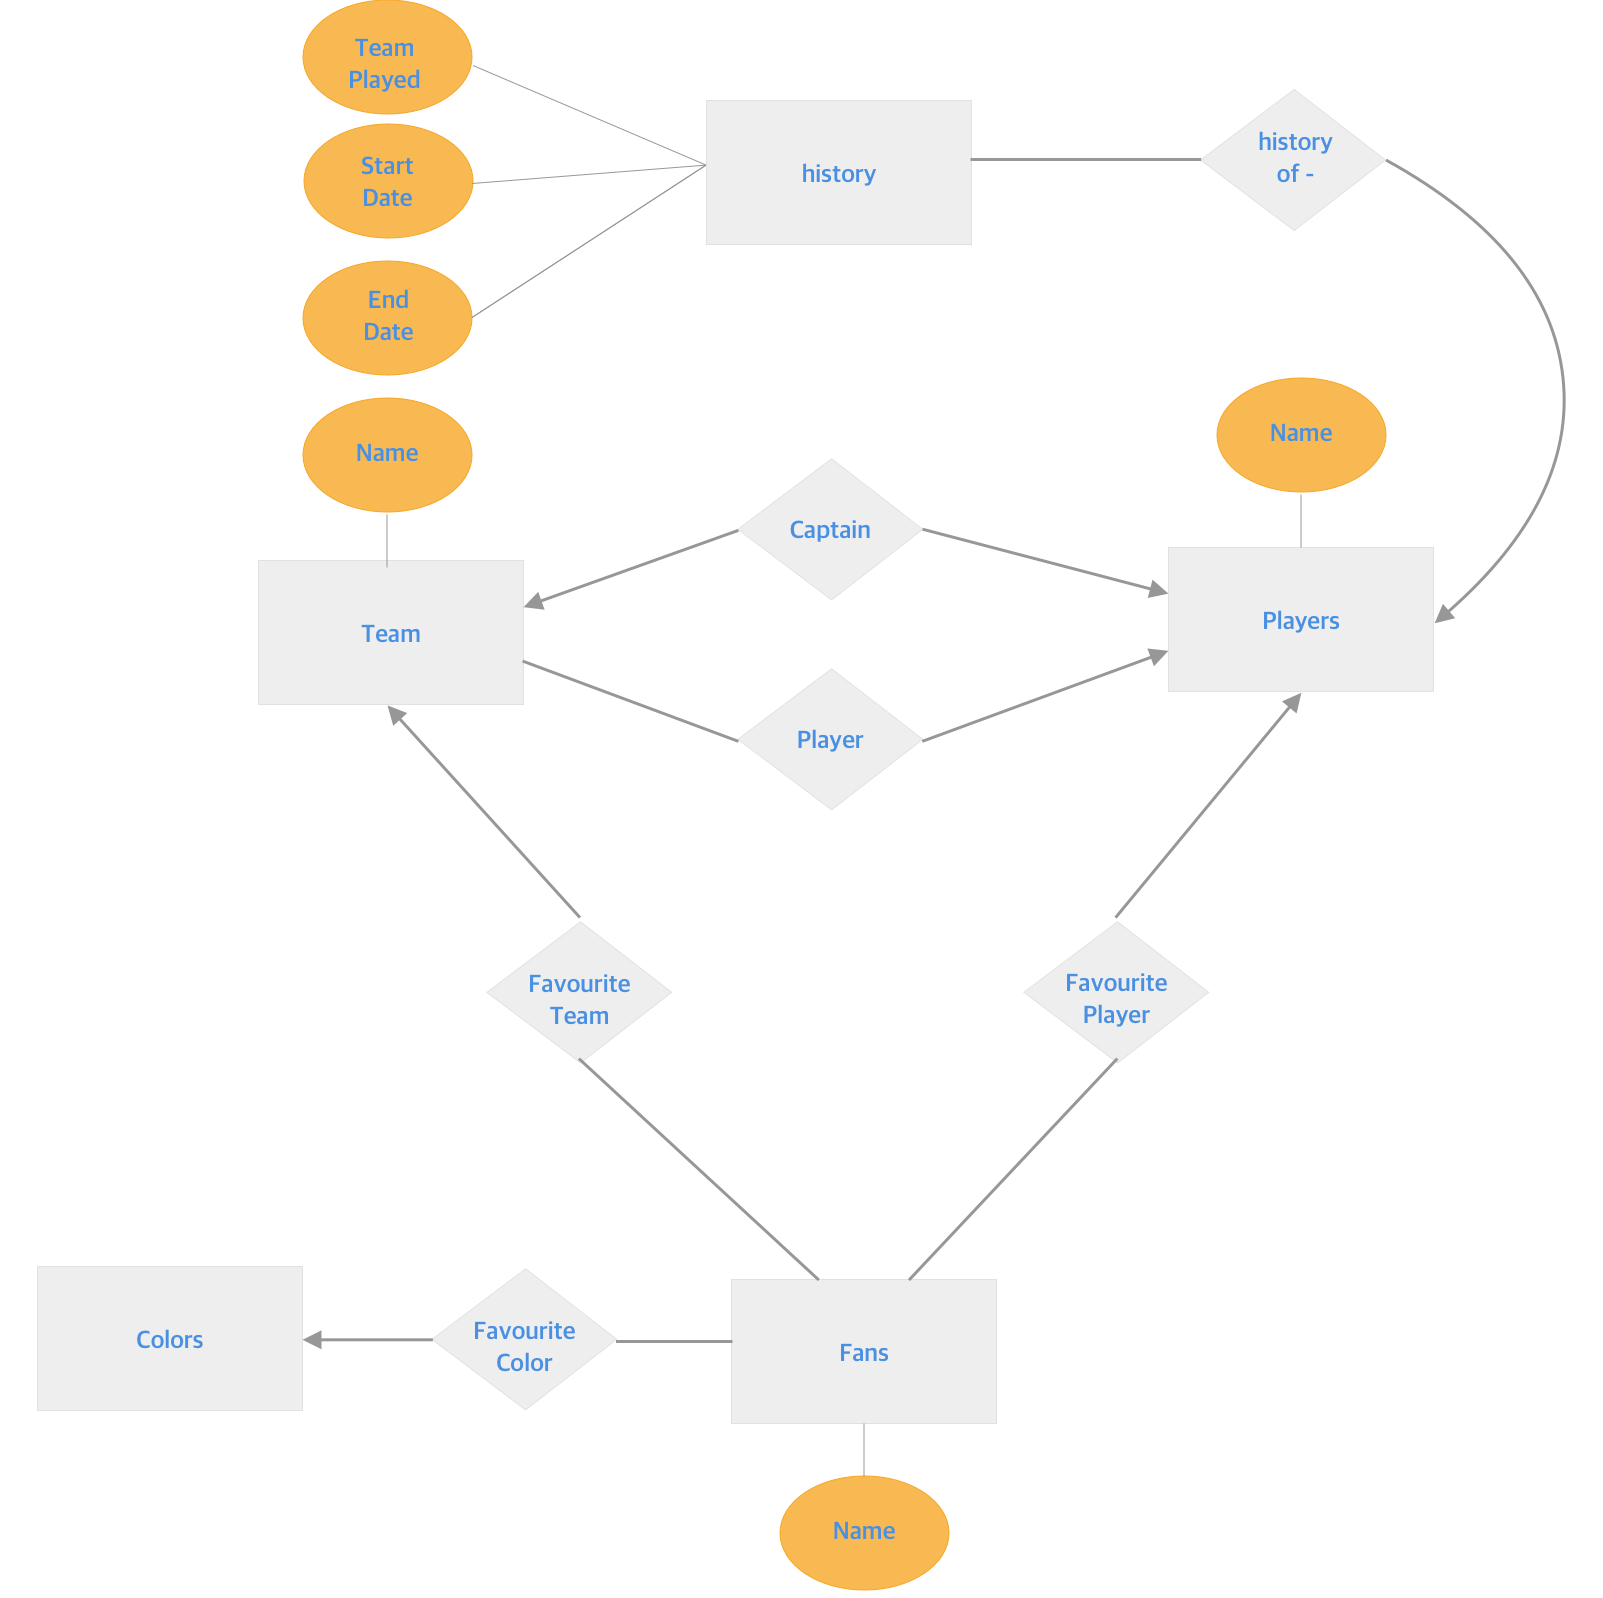
\includegraphics[width=\linewidth]{images/worksheet_14_solution_27.png}
    \end{center}

    \item

    \begin{center}
    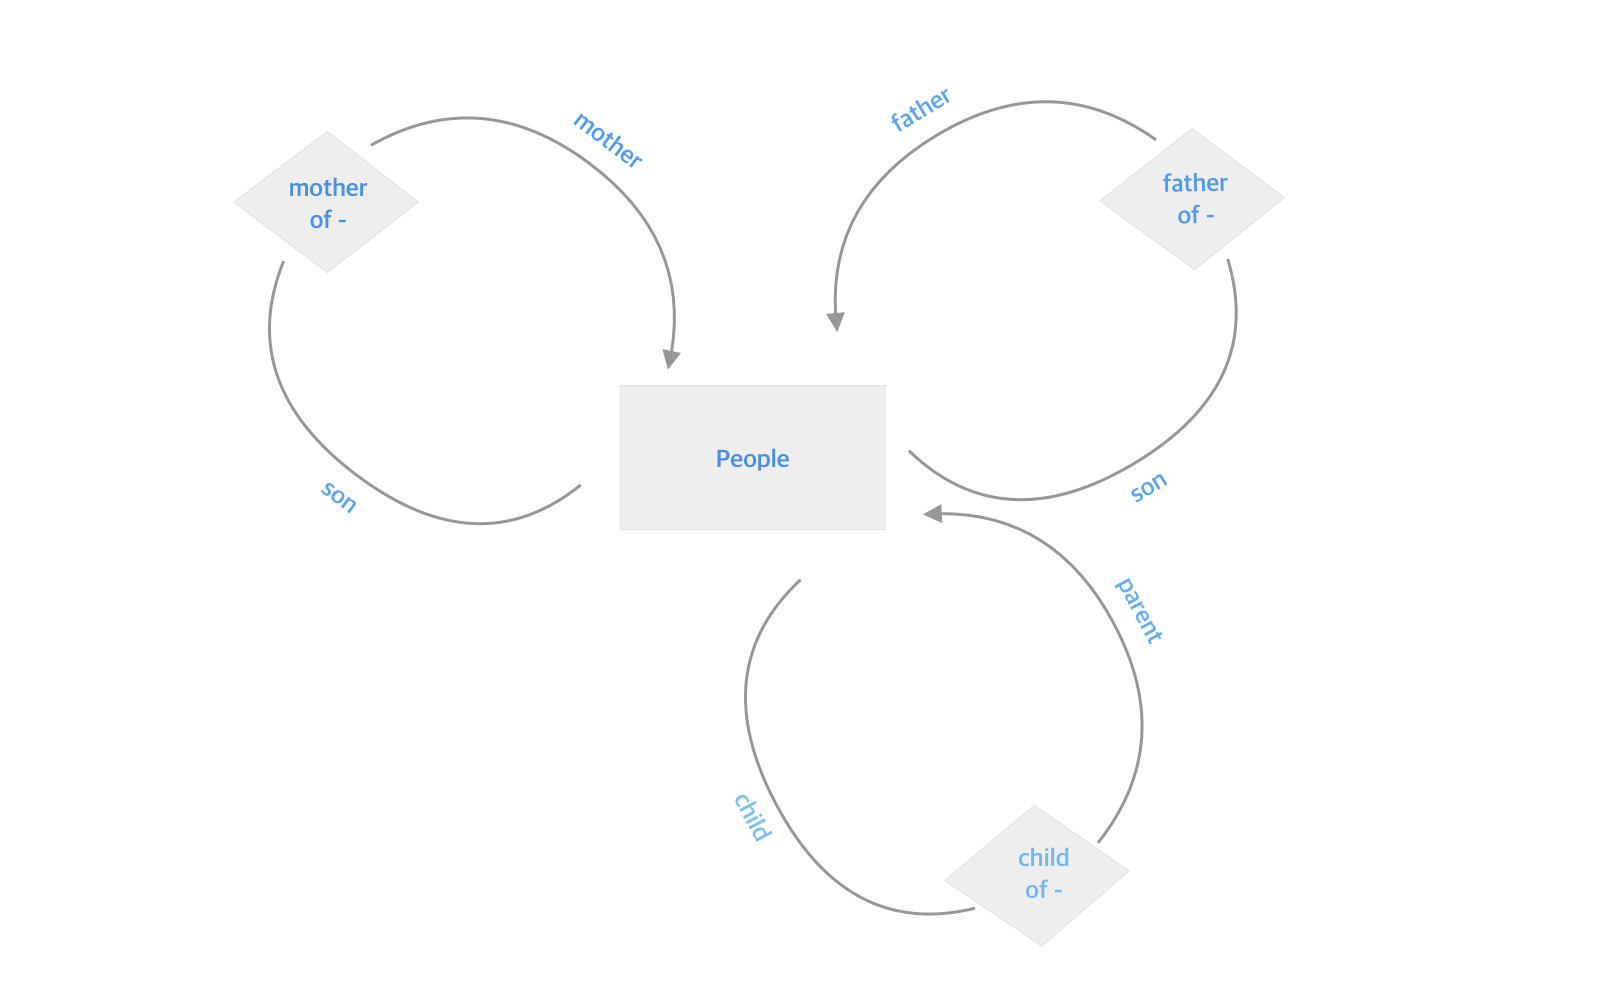
\includegraphics[width=\linewidth]{images/worksheet_14_solution_28.png}
    \end{center}


    \bigskip

    \begin{mdframed}
        \underline{\textbf{Correct Solution:}}

        \bigskip

        \begin{center}
        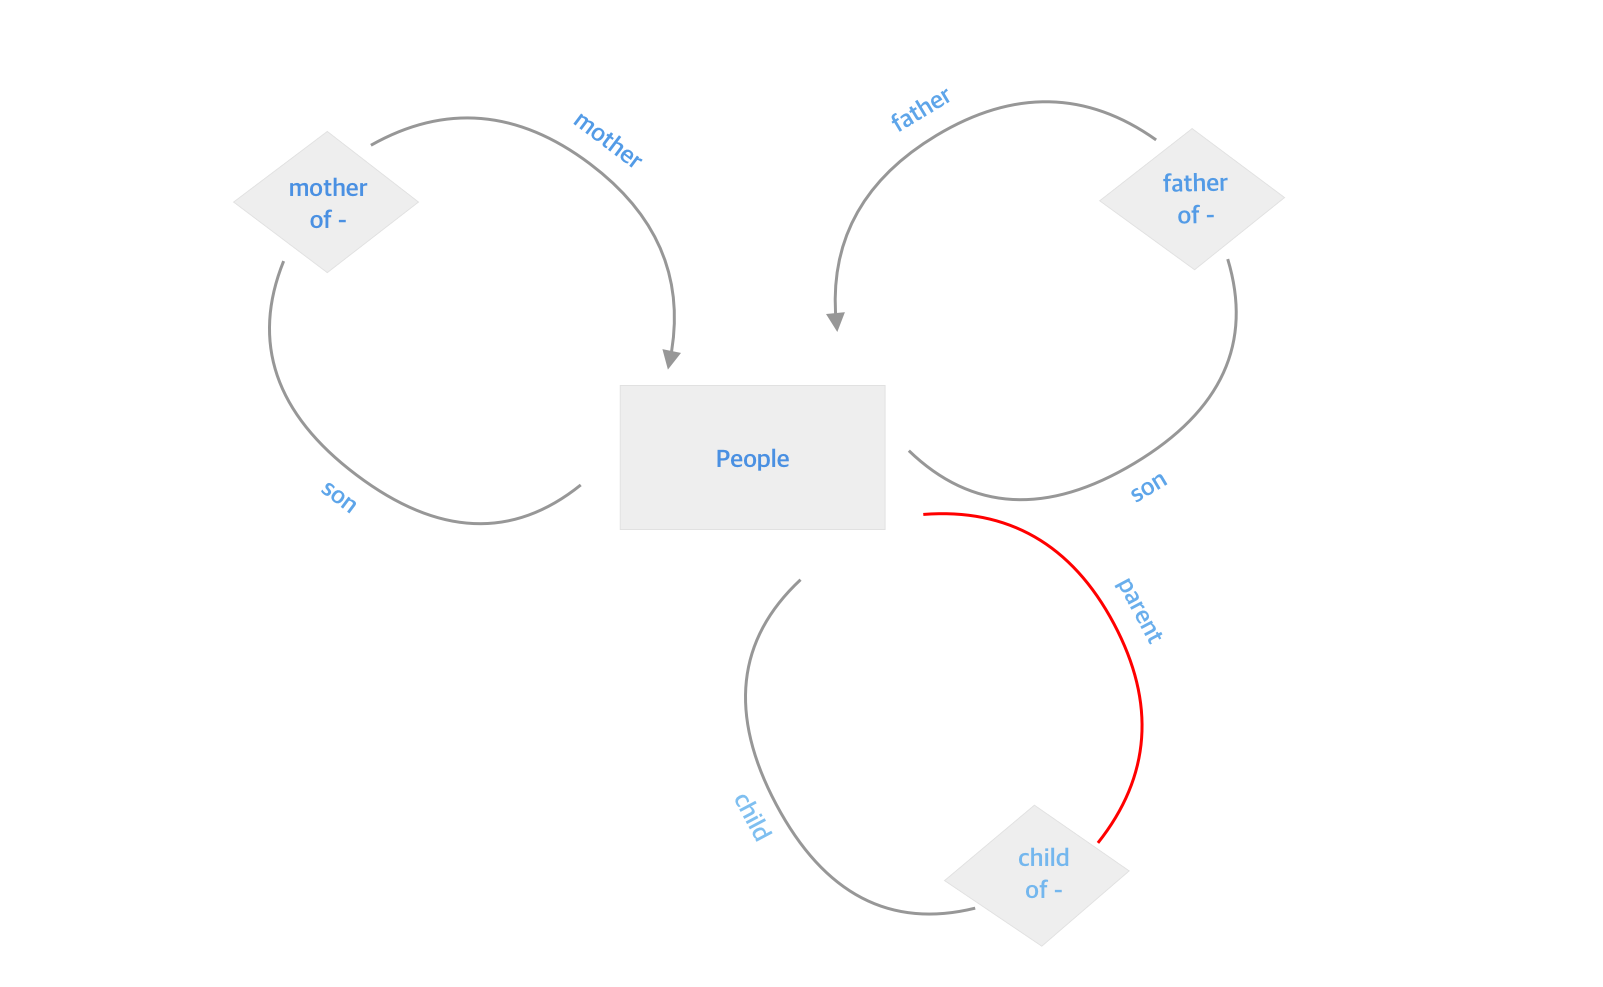
\includegraphics[width=\linewidth]{images/worksheet_14_solution_29.png}
        \end{center}
    \end{mdframed}

    \item

    \begin{center}
    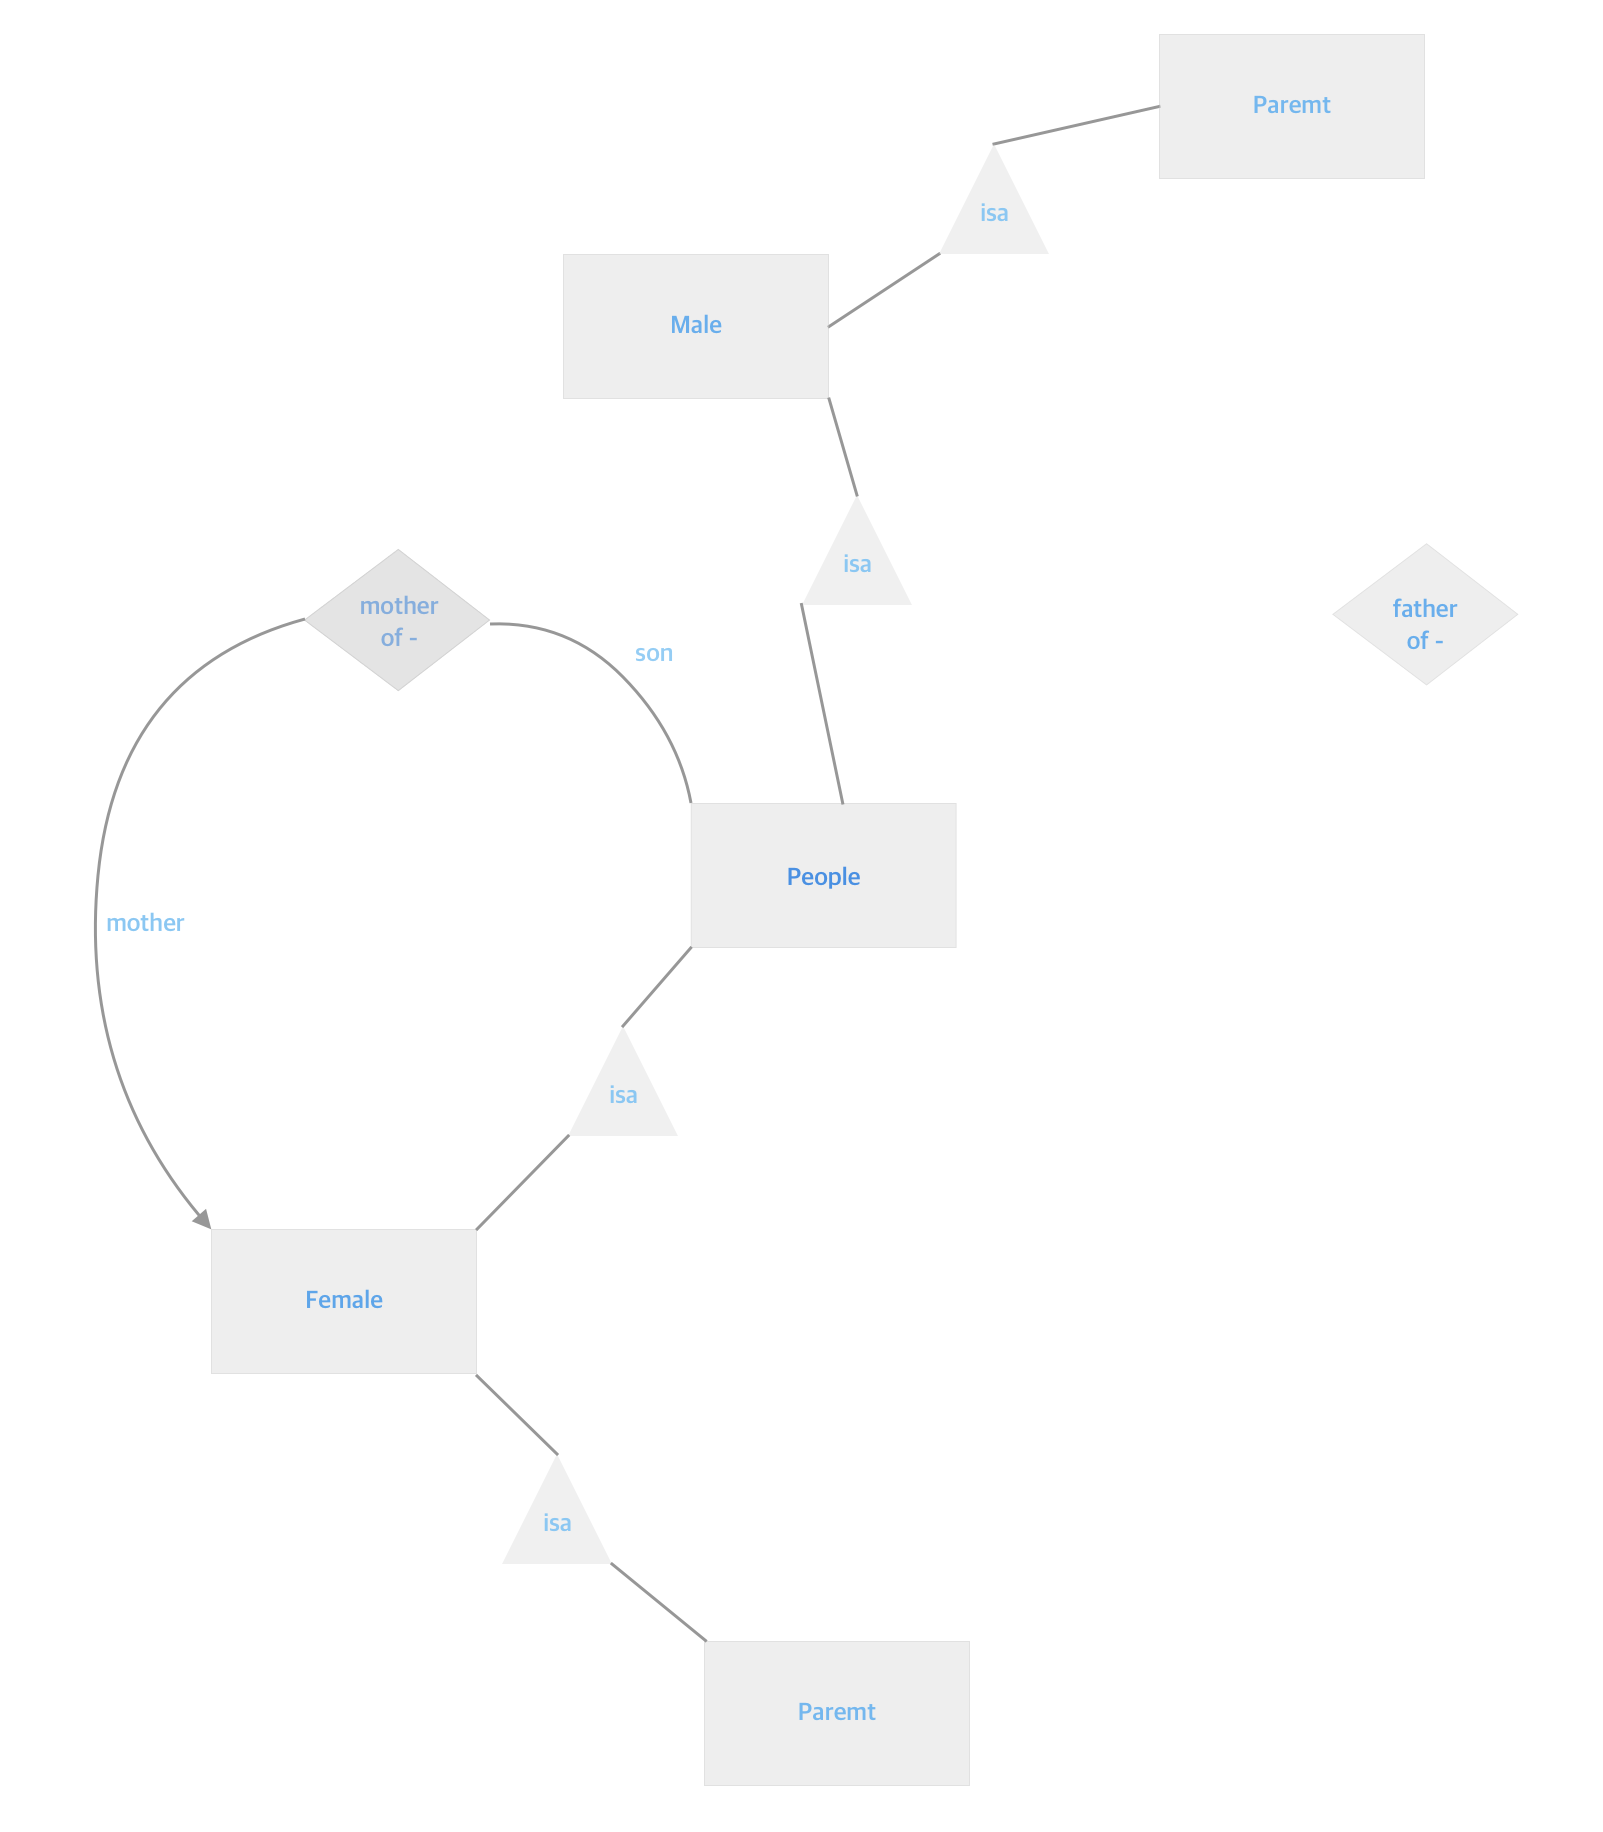
\includegraphics[width=\linewidth]{images/worksheet_14_solution_30.png}
    \end{center}

    \bigskip

    \underline{\textbf{Notes:}}

    \bigskip

    \begin{itemize}
        \item I feel the need to clarify with professor if two parent subclasses can
        exist
        \item I feel the need to ask professor whether this design is valid
    \end{itemize}

    \item

    \begin{enumerate}[a)]
        \item

        \begin{center}
        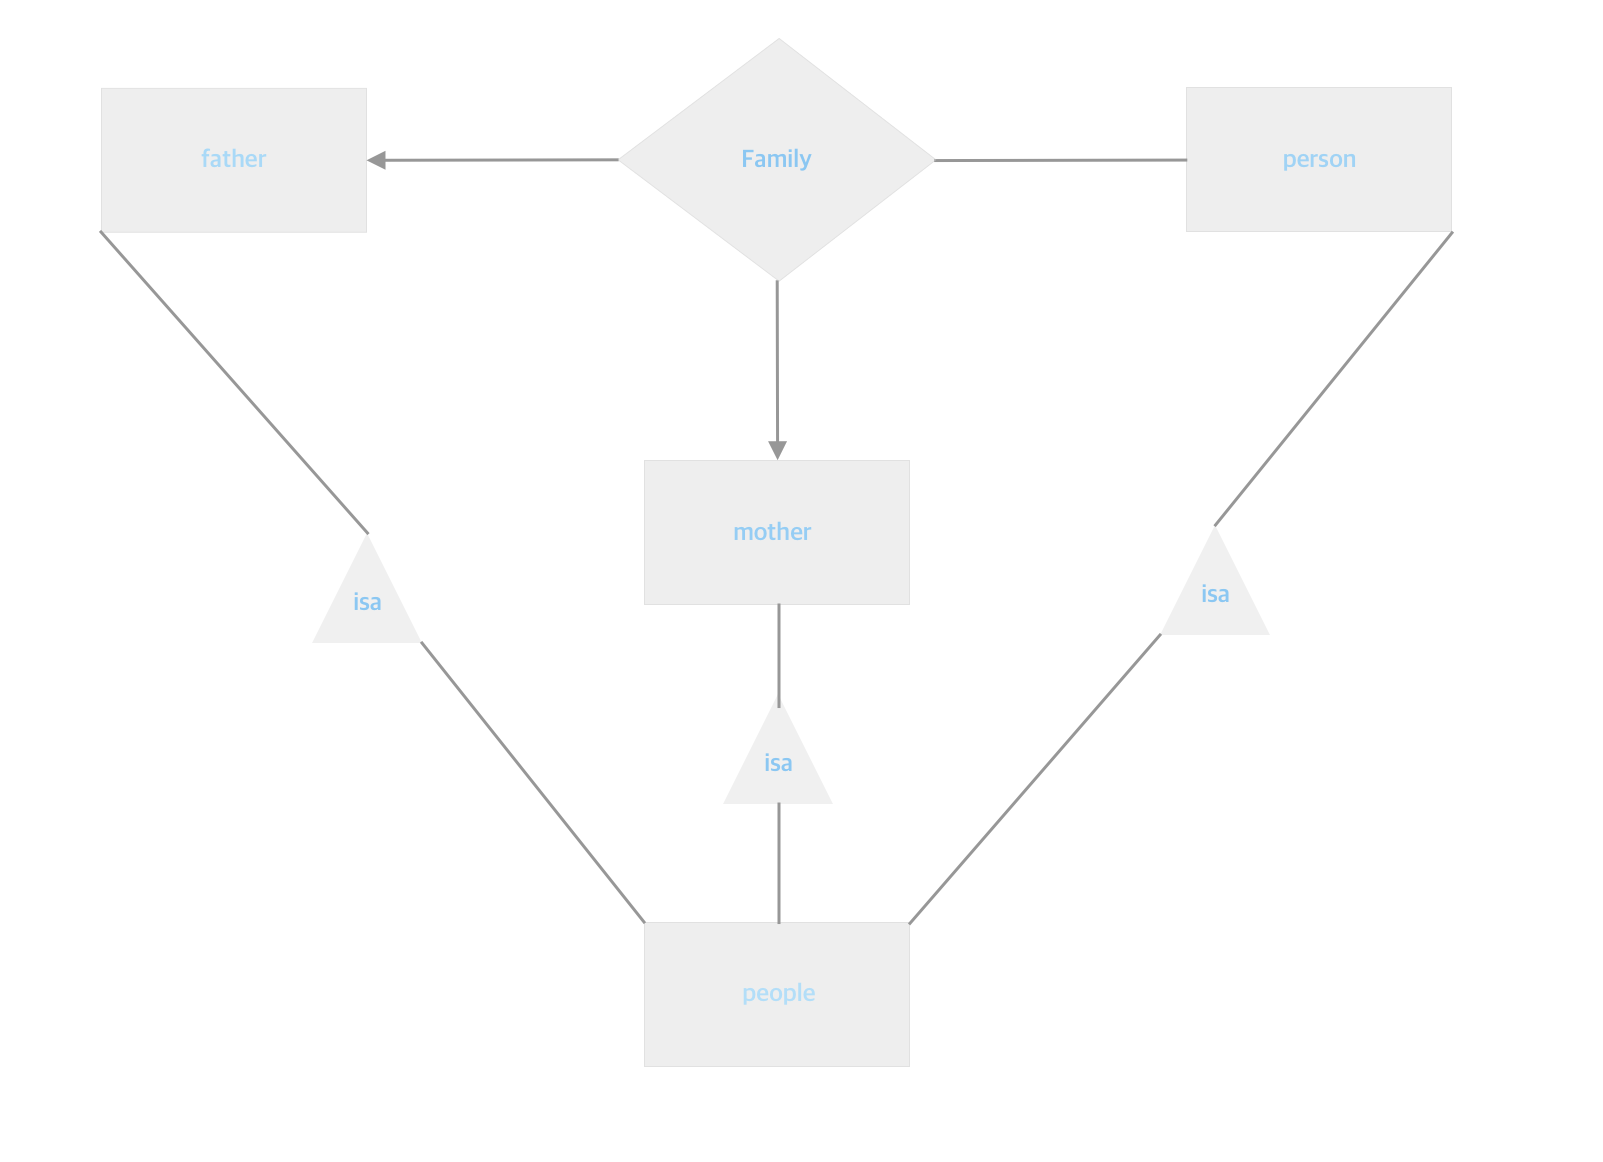
\includegraphics[width=\linewidth]{images/worksheet_14_solution_31.png}
        \end{center}

        \item

        \begin{center}
        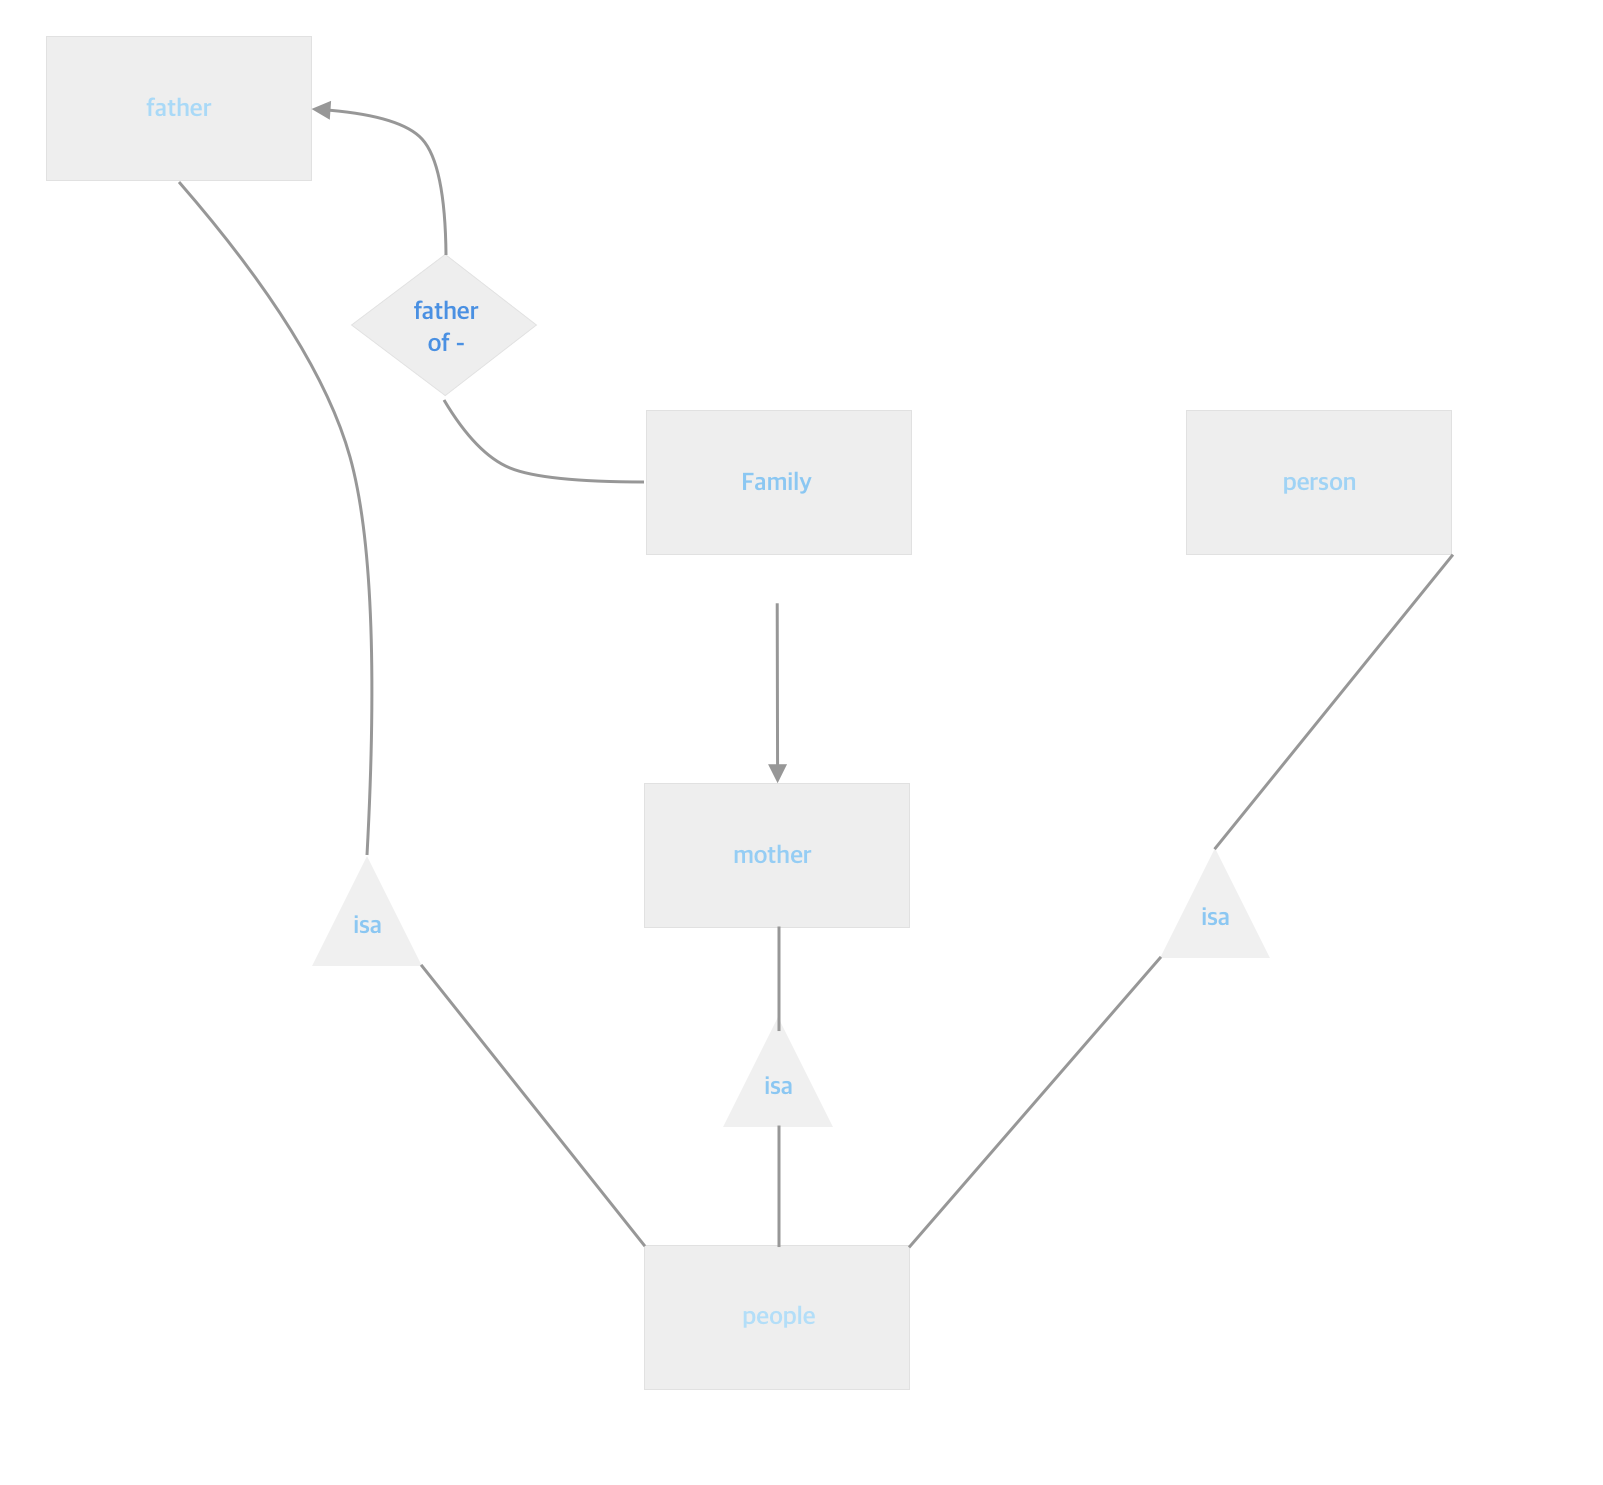
\includegraphics[width=\linewidth]{images/worksheet_14_solution_32.png}
        \end{center}

        \bigskip

        \underline{\textbf{Notes:}}

        \bigskip

        \begin{itemize}
            \item  I need to clarify with professor on one-to-many relationship.

            \bigskip

            Is it correct that the `one` side of `one-to-many' relationship represent
            foreign key in terms of SQL?

            \bigskip

            But how about the many side? What does it mean it to be many? so for example,
            ('Josh', 'Neville the father', 'Mary the mother'), ('Jay', 'Neville the father', 'Mary the mother'),
            is this one to many relationship?

            \bigskip

            In tabular terms / example what does one-to-many relationship represent
            in this context?
        \end{itemize}

    \end{enumerate}

    \item

    \begin{center}
    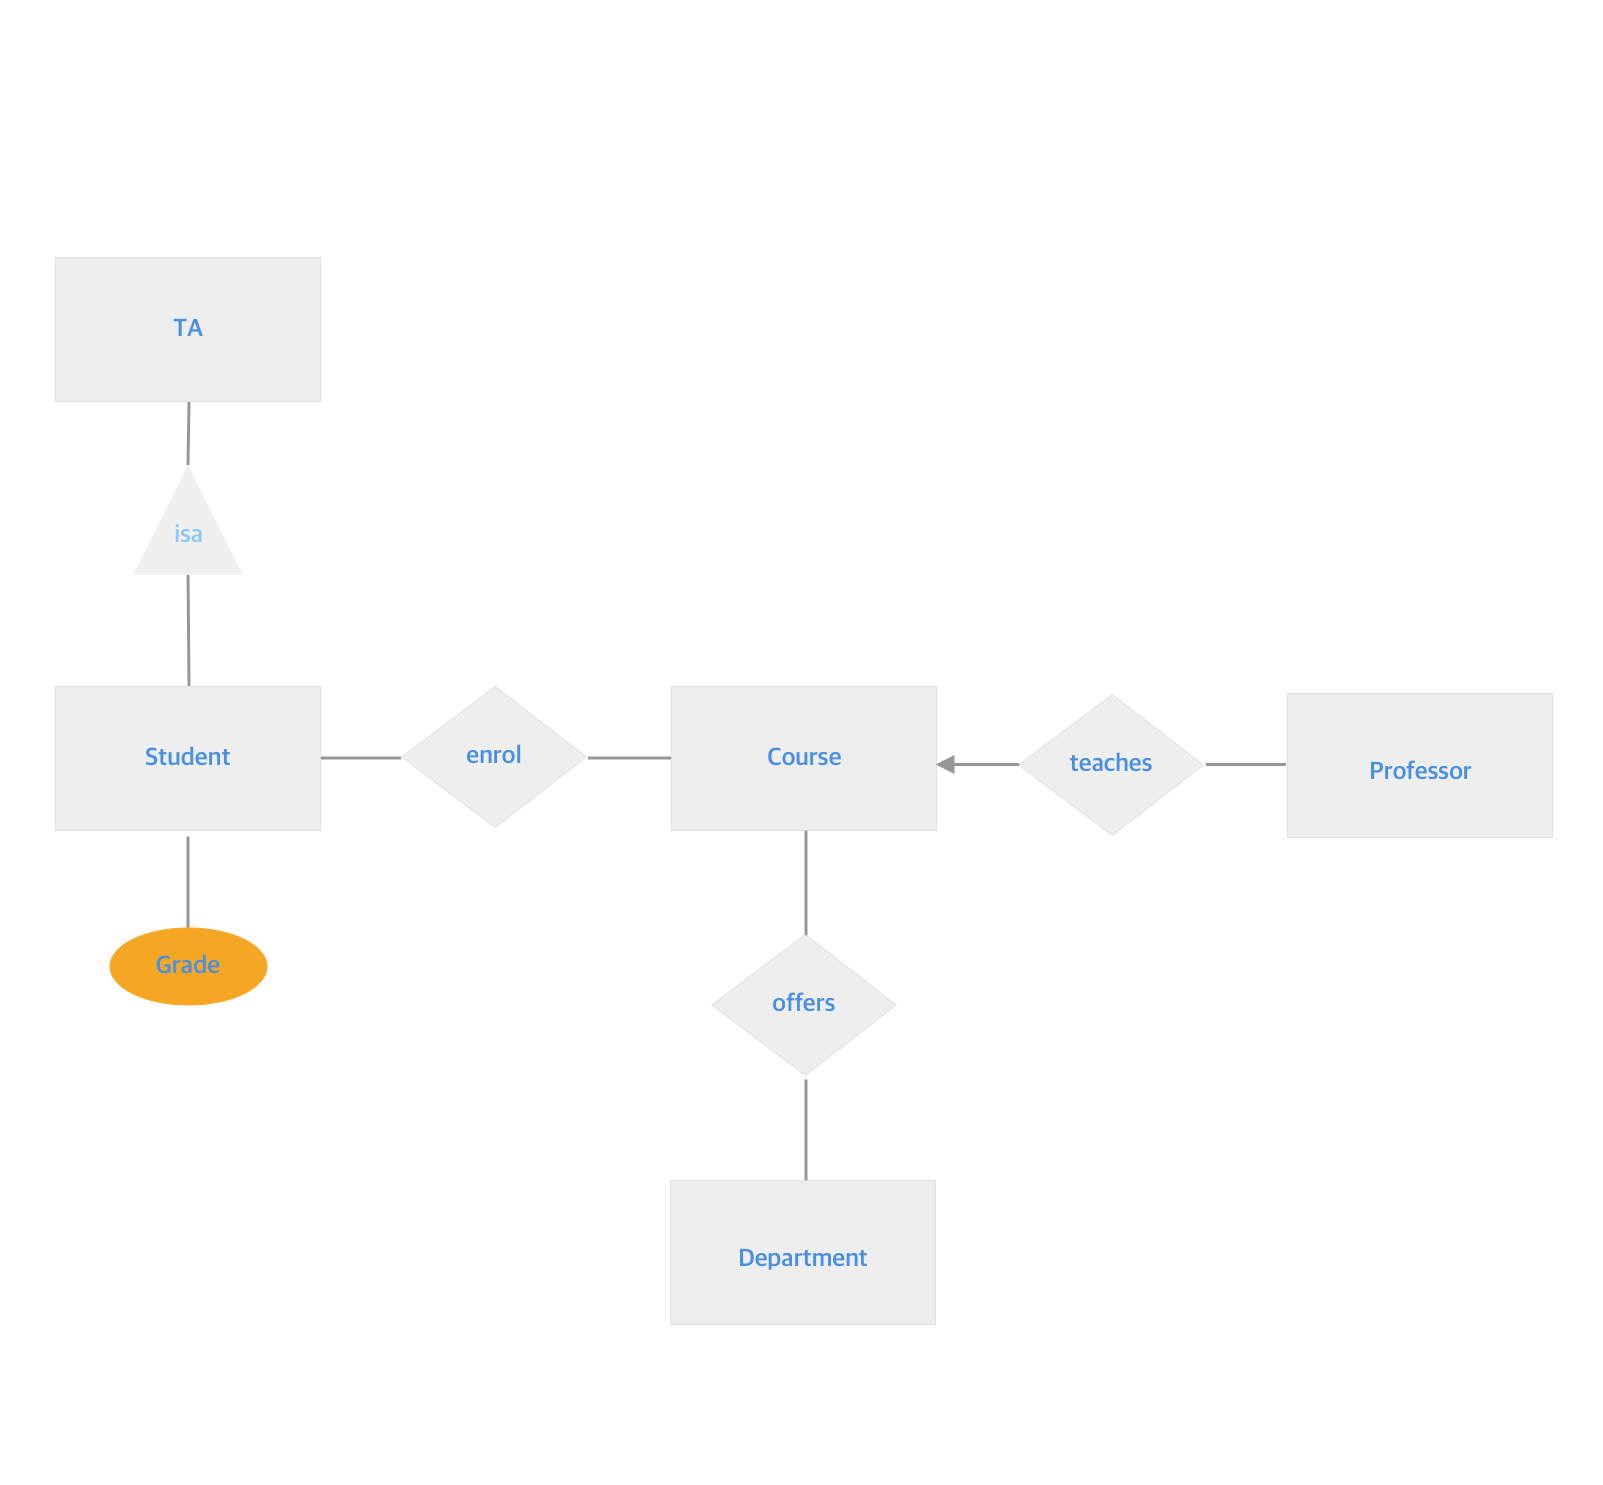
\includegraphics[width=\linewidth]{images/worksheet_14_solution_33.png}
    \end{center}

    \item

    \begin{center}
    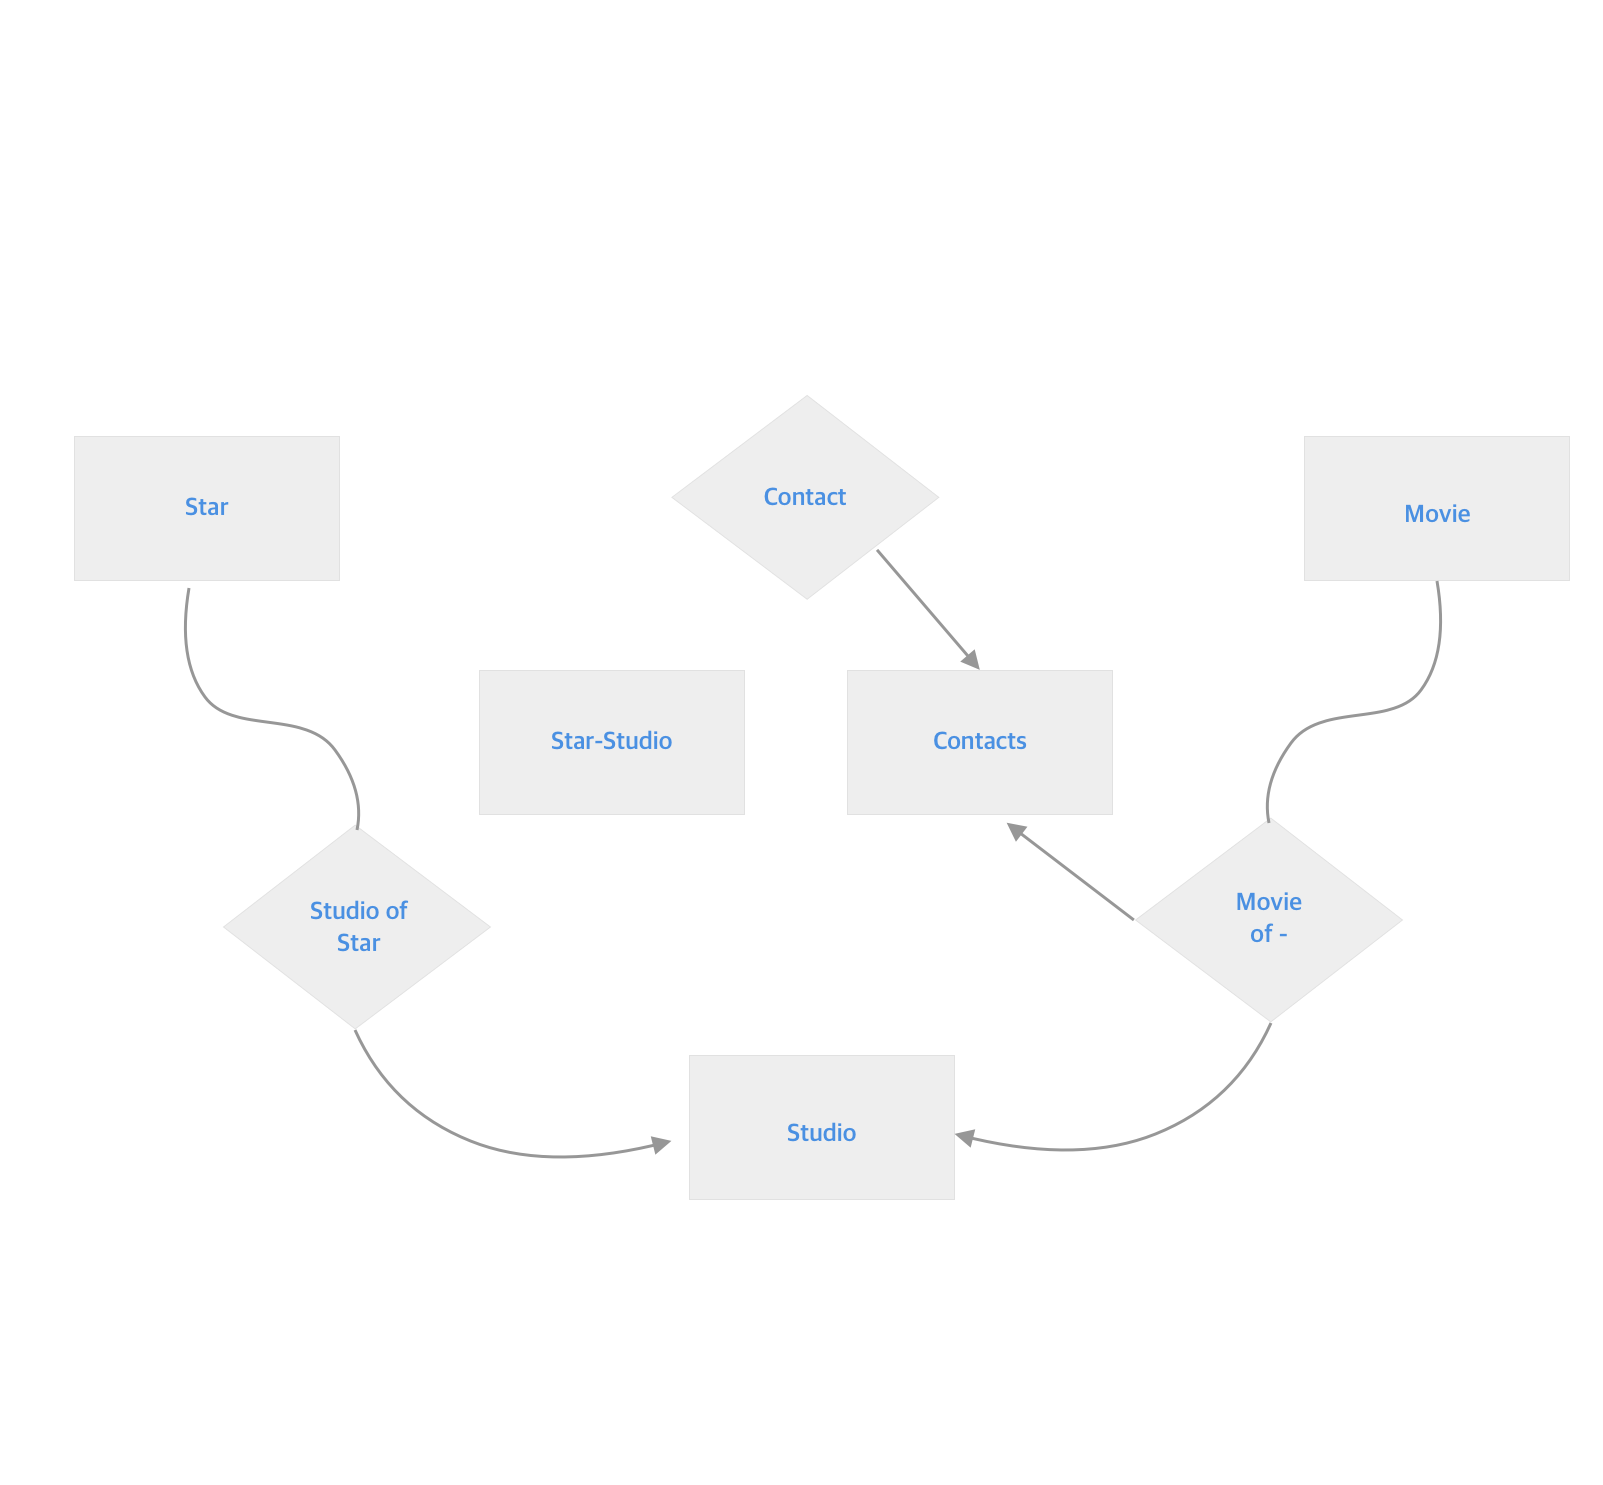
\includegraphics[width=\linewidth]{images/worksheet_14_solution_34.png}
    \end{center}

    \bigskip

    \begin{mdframed}
        \underline{\textbf{Correct Solution:}}

        \bigskip

        \begin{center}
        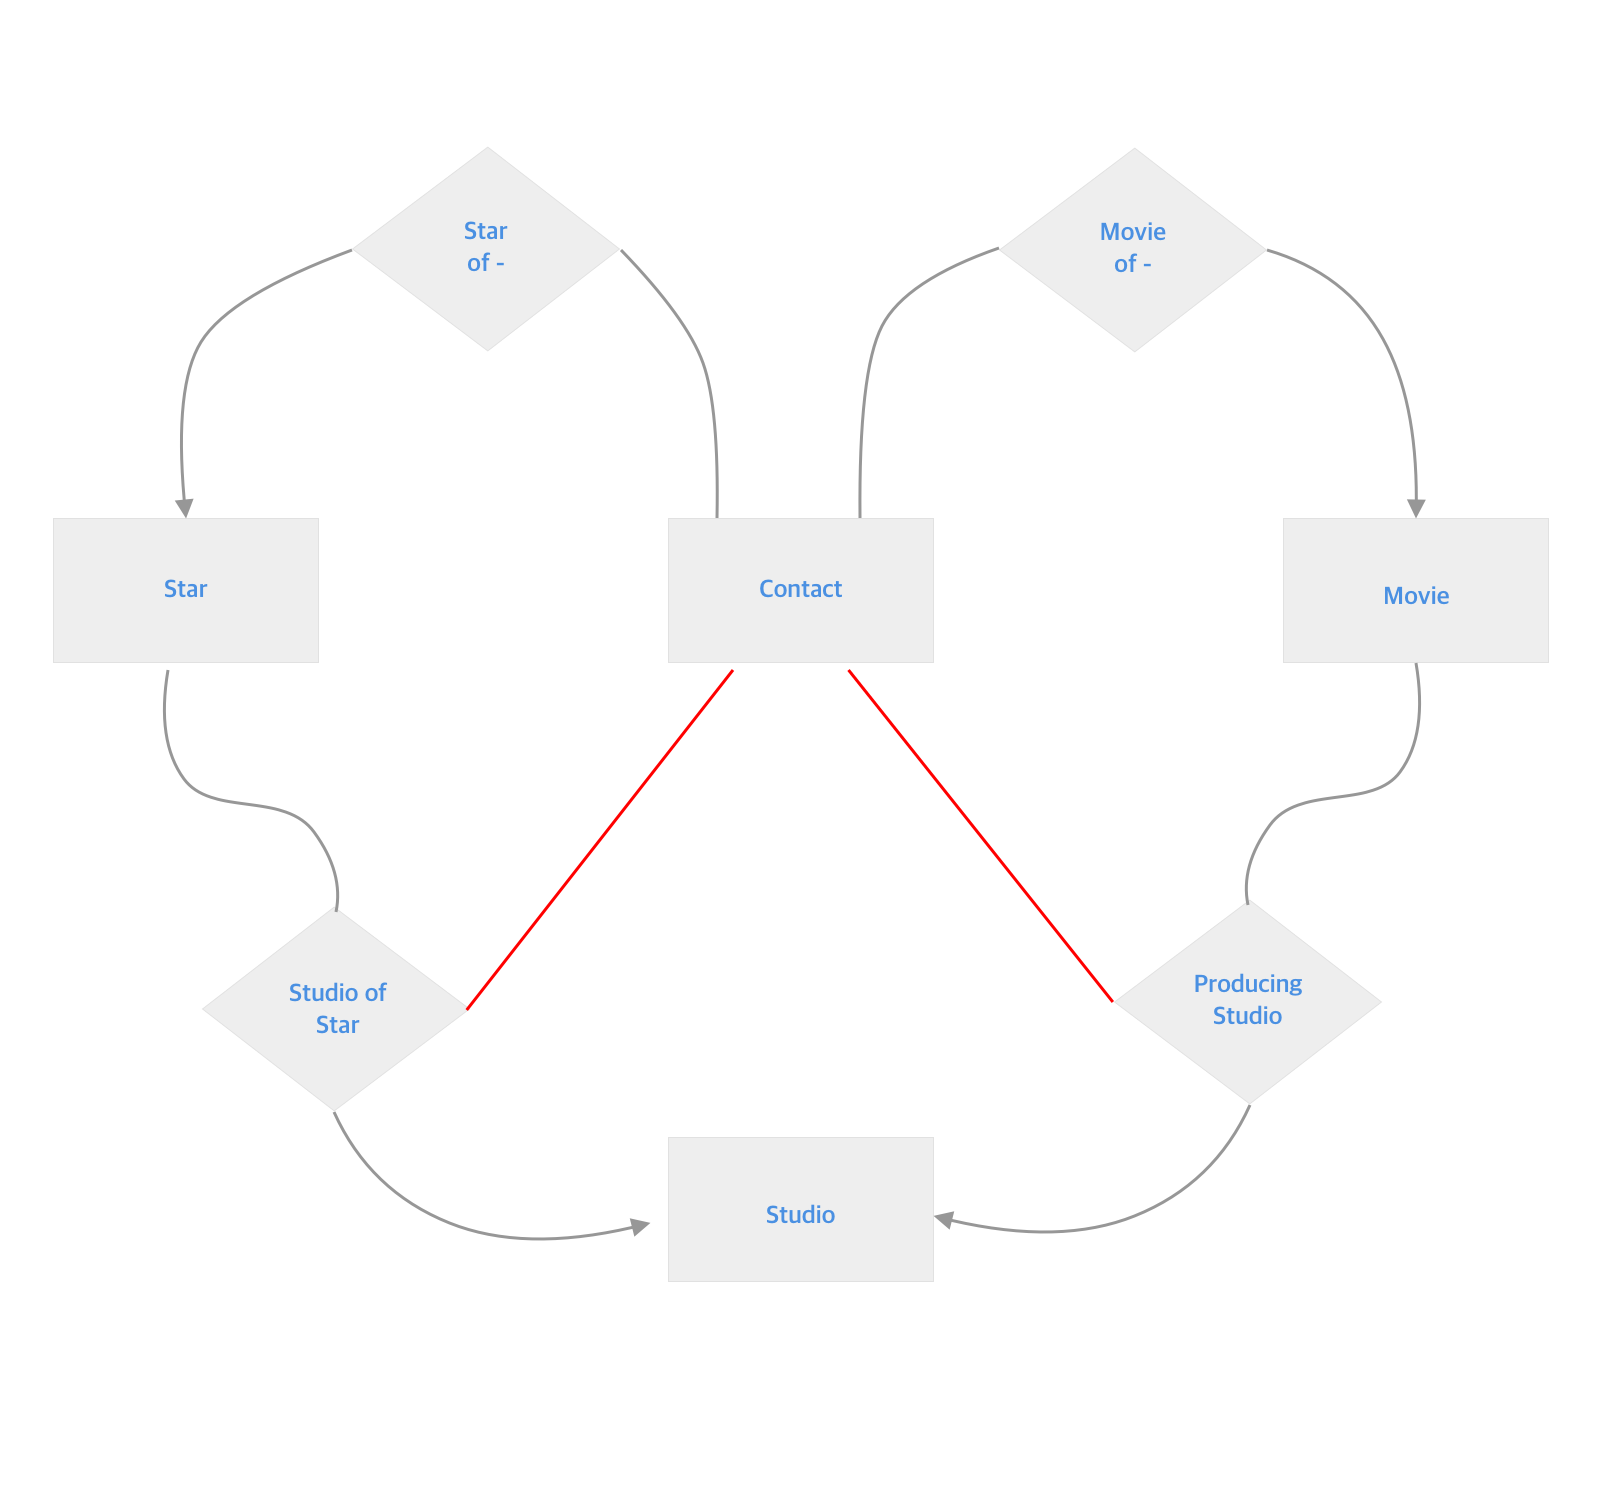
\includegraphics[width=\linewidth]{images/worksheet_14_solution_35.png}
        \end{center}

    \end{mdframed}

    \item

    \bigskip

    \underline{\textbf{Notes:}}

    \bigskip

    \begin{itemize}
        \item Design Principles

        \begin{enumerate}[1.]
            \item Faithfulness

            \begin{itemize}
                \item means design should make sense and meet its specification
                \item e.g. Adding attribute \textit{number-of-cylinders} to \textit{Stars} $\to$ NONO
            \end{itemize}

            \item Avoiding Redundancy

            \begin{itemize}
                \item \textit{Redundancy} means saying the same thing in
                two (or more) different ways
            \end{itemize}

            \bigskip

            \underline{\textbf{Example (The good example):}}

            \bigskip

            \begin{center}
            
\includegraphics[width=\linewidth]{images/worksheet_14_solution_36.png}
            \end{center}

            \bigskip

            \underline{\textbf{Example (The bad example):}}

            \bigskip

            \begin{center}
            
\includegraphics[width=\linewidth]{images/worksheet_14_solution_37.png}
            \end{center}

            \item Simplicty Counts

            \begin{itemize}
                \item Avoid adding more more elements than necessary
            \end{itemize}
            \item Choosing the Right Relationships

            \begin{itemize}
                \item Don't add relationships more than necessary
            \end{itemize}

            \item Picking the Right Kind of Element

            \begin{itemize}
                \item Don't add relationships more than necessary
            \end{itemize}
        \end{enumerate}
    \end{itemize}

\end{enumerate}

\end{document}